%%This is a very basic article template.
%%There is just one section and two subsections.
\documentclass[a4paper,12pt]{article} 
%\usepackage{a4wide}
%%\usepackage{a4}
\usepackage{setspace}
\onehalfspacing
\usepackage[utf8]{inputenc} 
\usepackage{graphicx}
%%\usepackage{hyperref}
 
\usepackage{amsmath}
\usepackage{framed}
 
\usepackage[german]{babel}  %% ngerman für neue eher nicht
 

\usepackage{url}

\usepackage{microtype}

\usepackage{pdfpages}

\usepackage{geometry}
\geometry{a4paper,left=25mm,right=25mm, top=25mm, bottom=25mm} 

 
%%%%%%%%%%%%%%%%%%%%%%%%%%%%%%%%%%%%%%%%
\usepackage{color}
\usepackage{listings}
\lstset{ %
language=C++,                % choose the language of the code
basicstyle=\footnotesize,       % the size of the fonts that are used for the code
%%numbers=left,                   % where to put the line-numbers
%numberstyle=\footnotesize,      % the size of the fonts that are used for the
% line-numbers
%stepnumber=1,                   % the step between two line-numbers. If it is 1
% each line will be numbered
%numbersep=5pt,                  % how far the line-numbers are from the code
backgroundcolor=\color{white},  % choose the background color. You must add \usepackage{color}
showspaces=false,               % show spaces adding particular underscores
showstringspaces=false,         % underline spaces within strings
showtabs=false,                 % show tabs within strings adding particular underscores
frame=single,           % adds a frame around the code
tabsize=2,          % sets default tabsize to 2 spaces
captionpos=b,           % sets the caption-position to bottom
breaklines=true,        % sets automatic line breaking
breakatwhitespace=false,    % sets if automatic breaks should only happen at whitespace
escapeinside={\%*}{*)}          % if you want to add a comment within your code
}
%%%%%%%%%%%%%%%%%%%%%%%%%%%%%%%%%%%%%%%%

\renewcommand{\figurename}{Bild}
\renewcommand{\contentsname}{Inhaltsverzeichnis}
\begin{document}


\begin{figure}[htbp]
\centering

\includegraphics[scale=0.4]{Umit_logo.jpg}
\label{figure_deckblatt}
\end{figure}


\thispagestyle{empty}   %% style nur für die erste seite definieren
\begin{center}
\textbf{ \LARGE{Algorithmische Optimierungen für iterative
Dekonvolutionsverfahren \par }}
\end{center}


\begin{verbatim}
\end{verbatim}

\begin{center}
Bachelorarbeit\\
zur Erlangung des akademischen Grades\\
\Large{Bachelor of Science (BSc.)} \\
\end{center}

\begin{center}
im Rahmen des \\
Bachelorstudiums\\
Biomedizinische Informatik
\end{center}


\begin{verbatim}
\end{verbatim}



\begin{center}
vorgelegt von: \\
\textbf{\Large{Ing. Martin Erler}}
\end{center}


\begin{verbatim}
\end{verbatim}


\begin{center}
betreut von:\\
a.o. Univ.-Prof. Dr. Martin Welk
\end{center}

\begin{center}
an der:\\
UMIT - Private Universität für Gesundheitswissenschaften,\\
Medizinische Informatik und Technik
\end{center}



\newpage
\tableofcontents
\newpage

%%%%%%%%%%%%%%%%%%%%%%%%%%%%%%%%%%%%%%%%%%%%%%%%%%%%%%%%%%%%%%%%%%%%%%
%%%%%%%%%%%%%%%%%%%%%%%%%%%%%%%%%%%%%%%%%%%%%%%%%%%%%%%%%%%%%%%%%%%%%%
 


\section{Einleitung und Stand der Forschung}
\subsection{Dekonvolution in der Bildverarbeitung}



Dekonvolutionsverfahren haben das Ziel die Faltungsoperation (Konvolution)
umzukehren. Eine solche Faltungsoperation erfolgt implizit bei der Aufnahme
eines Bildes. Jedes Mal wenn wir ein Foto aufnehmen, kann
diese Bildaufnahme mathematisch als Konvolution modelliert werden. Diese Faltung
kann auch mit einer ungewünschten Funktion ablaufen. Dann entsteht ein
unscharfes Bild. Die Dekonvolution verfolgt das Ziel, diese Faltung mit der
sog. Punktbildfunktion rückgängig zu machen. Wenn die Parameter bekannt sind,
kann man also aus dem unscharfen Bild ein scharfes berechnen.

Unscharfe Bilder können auf verschiedene Weise entstehen: Wenn die
Belichtungszeit im Verhältnis zur Objektbewegung zu lange dauert, entsteht 
Bewegungsunschärfe. Wir kennen das Problem, wenn wir im Dunkeln fotografieren
und das Bild "`verwackelt"' abgelichtet wird. Es kann ebenso passieren, dass die
Entfernungseinstellung falsch vorgenommen wurde. Die Fokussierung klappt also
nicht und das Ergebnis ist, dass das gewünschte Objekt unscharf dargestellt wird.
Die wichtigsten Systemparameter sind bei der Bildaufnahme die
Belichtungszeit, die Sensor- oder Filmempfindlichkeit, die Brennweite, der
Brennpunkt oder Fokus und die Geschwindigkeit der abzubildenden
Objekte.

Je genauer diese Parameter bekannt sind, desto besser läßt sich die Faltung
durch die Dekonvolution rückgängig machen. Man unterscheidet verschiedene Typen
der Dekonvolution. Eine wichtige Unterscheidung ist, ob und wie genau die
Punktbildfunktion bekannt ist. Die blinde Dekonvolution hat das Ziel, die
Faltung ohne genaue Kenntnis der Punktbildfunktion rückgängig zu machen. Die Art
und das Ausmaß der Unschärfe sind also unbekannt. Eine weitere Unterscheidung
der Verfahren bringt die Ortsvarianz der Punktbildfunktion. Die Unschärfe kann über
das gesamte Bild gleich sein, oder auch nur einzelne Bildbereiche betreffen. Bei
einer über den gesamten Bildbereich gleichbleibenden Unschärfe spricht man von
einer ortsinvarianten Faltung, bzw. Dekonvolution. Bei einer ortsabhängigen
Unschärfe, wenn also nur einzelne Bereiche oder Objekte unscharf dargestellt
werden, muss die ortsvariante Dekonvolution angewendet werden.

Dekonvolutionsverfahren werden meist schrittweise, also iterativ durchgeführt.
Es gibt aber auch nicht iterative Dekonvolutions\-algorithmen. Bei der Iteration
wird die Schärfe dann Schritt für Schritt entfernt oder reduziert. Wenn der
Algorithmus über Regularisierungsparameter verfügt, kann der Grad dieser
Abminderung parametriert werden. Das macht dann Sinn, wenn ungewünschte
Artefakte eine beliebig starke Schärfung verhindern. 

%%In der praktischen
%%Anwendung spielt das eine große Rolle, da praktisch jedes Bild einen 
%%konkreten Rauschpegel aufweist.


%%\textbf{Übersicht}. 
%%\textbf{blinde, nicht-blinde Dekonvolution}. wird hier kurz erklärt\\
%%\textbf{ortsvariant, ortsunabhängig}. wird hier kurz erklärt\\


\subsection{Modellierung von Bildern und Unschärfe} \label{chp:einf_unschaerfe}

\subsubsection{Bildmodellierung}

\textbf{Bild als Funktion}. 
Ein Bild läßt sich als Funktion beschreiben:

\begin{equation} \label{eq:discrete}
f: \Omega \to R
\end{equation}


Dabei stellt $\Omega$ den Bildbereich oder die Bildebene dar.
$R$ beschreibt den Wertebereich. Wir beschränken uns auf Grauwertbilder. 


\textbf{Faltung}. Wir führen nun Faltungsoperator ein. Dabei repräsentiert
$f(x)$ das gefaltete Bild:

\begin{equation} \label{eq:faltung1}
f(x)=\int_\Omega{H(x,y) \cdot g(y)dy+n(x)}
\end{equation}

Als $g(x)$ bezeichnen wir das gedachte ideale Bild. Und $H(x,y)$ bezeichnen wir
als Faltungskern, oder Punktbildfunktion
(engl.: Point Spread Function, PSF). Sie beschreibt die Art und Weise, wie das
ursprüngliche (gedachte) Bild verwischt worden ist. $n(x)$ beschreibt
hier den Einfluss von Rauschen bei der Bildaufnahme. Wenn wir die Operation invertieren können, ist es also möglich
mit Kenntnis der PSF auf das gedachte ideale Bild ohne Unschärfe zu gelangen. Da
wir aber $n(x)$ nicht kennen, sprechen wir in der Folge von einem schlecht
gestellten inversen Problem.
Wenn die PSF über $\Omega$ gleich bleibt, liegt eine ortsunabhängige Faltung
vor und wir erhalten (\ref{eq:faltung2}).

\begin{equation} \label{eq:faltung2}
f(x)=(g*h)(x)+n(x)
\end{equation}

\begin{itemize}
  \itemsep -1pt
  \item $f$ beaobachtetes, unscharfes Grauwertbild
  \item $g$ gewünschtes, scharfes Grauwertbild
  \item $n$ Bildstörungen (Rauschen)
  \item $h$ ortsunabhängige Punktbildfunktion (PSF)
  %%\item $\Omega$ Bildebene
\end{itemize}

Diese Modellierung gilt nun auch nach der Abtastung (Sampling). Wir haben
ein digitales Bild vorliegen. Dabei ist nun die Bildebene $\Omega$ diskretisiert und 
besteht aus Pixeln. $R$ stellt den diskretisierten Wertebereich dar 
und wird bei uns auf 8 bit, also einen Bereich von
$0\ldots255$ beschränkt. 

\begin{figure}[htbp]
\centering
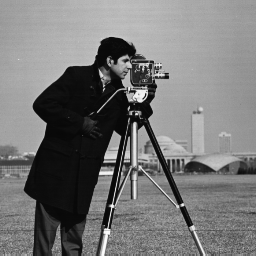
\includegraphics[scale=0.8]{camera.png}
\caption{Ausgangsbild}
\label{figure_camera}
\end{figure}


\subsubsection{Bewegungsunschärfe} 
Bewegungsunschärfe entsteht durch Objekt- oder Kamerabewegung während der
Bildaufnahme. Wenn diese Bewegung im Verhältnis zur Belichtungszeit zu schnell
abläuft, entsteht eine Unschärfe in Bewegungsrichtung. \\
 \textbf{Ortsvariante, -invariante Bewegungsunschärfe.} Die Unschärfe
 kann ortsabhängig oder auch ortsinvariant sein. Bei der ortsinvarianten
 Unschärfe werden alle Pixel im Bild gleich verwischt.
 Ein praktisches Beispiel ist die Bildaufnahme ohne Stativ: Die Kamera
 bewegt sich während der Bildaufnahme ( die Rotation wird ausgeschlossen,
 oder vernachlässigt).
 Bei einer ortsvarianten Unschärfe ändert sich der Faltungskern. Unschärfe variiert im Bild. Das kann
 durch Objektbewegung passiert sein: Beispielsweise wenn ein Auto durch das Bild
 fährt, kann es unscharf abgebildet werden. Die entstandene Unschärfe betrifft
 nur das Auto. Die anderen Pixel sind scharf abgebildet. Man spricht dann von einer
 ortsvarianten PSF.\\
\textbf{Konstante oder veränderliche Unschärfe?} In dem gezeigten Bild liegt
also ein Boxfilter zugrunde. Alle Pixel des Faltungskerns haben denselben (konstanten)
Grauwert. Die Kamera- oder Objektbewegung war in diesem Falle konstant. Wenn die Bewegung mit
einer veränderlichen Geschwindigkeit $v$ erfolgt, entsteht eine nicht konstante
Bewegungsunschärfe.

\textbf{Boxfilter 1D}
Der sogenannte eindimensionale Boxfilter kannn besonders effizient berechnet
werden. Ein Beispiel eines solchen Filters zeigt die Abb. \ref{figure_motion}. 
Er ist konstant (alle Grauwerte haben den selben Wert) und verläuft 
exakt horizontal oder vertikal. Der Boxfilter wurde bereits im Jahre 1981
von McDonnell beschrieben \cite{mcdonnell}.
 
\begin{figure}[htbp]
\centering
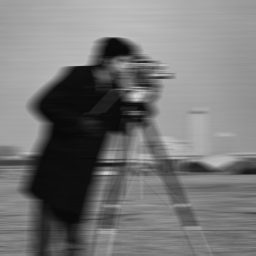
\includegraphics[scale=0.8]{move17.png}

\includegraphics[scale=2.1]{kern1D37px.png}
\caption{1D Boxfilter mit 17 Pixel Ausdehnung in horizontaler Richtung, rechts
unten ist der vergrößerte Faltungskern zu erkennen}
\label{figure_motion}
\end{figure}



\subsubsection{Boxfilter 2D}
Das Bild \ref{figure_motion2d} zeigt das Ergebnis, bei einer Faltung mit einem
zwei-dimensionalen Boxfilter. Alle besetzten Pixel der PSF haben den gleichen
Grauwert.
Im Gegensatz zu den anderen hier gezeigten Faltungskernen hat der
2D-Boxfilter eine geringere praktische Bedeutung. Die Unschärfe aus Bild
\ref{figure_motion2d} kommt physikalisch nicht vor und ist synthetisch erzeugt.


\begin{figure}[htbp]
\centering
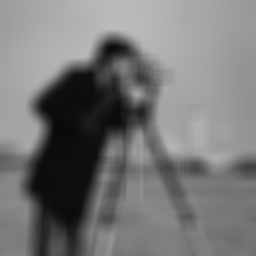
\includegraphics[scale=0.8]{box17.png}

\includegraphics[scale=7]{kern2D9mal9.png}
\caption{2D Boxfilter mit 17 Pixel Unschärfe, rechts daneben der Faltungskern,
vergrößert}
\label{figure_motion2d}
\end{figure}


\subsubsection{Lensblur, Defokussierung}

Der Lensblurfilter ist von besonderer praktischer Bedeutung: Er generiert ein
Bild, das einer fehlerhaften Fokussierung entspricht. Der Kern dieses Filters
ist ein gefüllter Kreis. Das Bild \ref{figure_confusion} illustriert, wie der Radius und die
entstehende Unschärfe optisch zusammenhängen. Die Form der PSF rührt von der
Form der Blende her. Im Objektiv der Kamera hat die Blendenöffnung eine
annähernd kreisrunde Öffnung. Je nach Objektiv kann die Blende aber auch einem
Polygon ähnlich sein. Wenn man das optische System eines
Objektivs weiter betrachtet, lässt sich festhalten, dass der Brennpunkt idR. über den Bildbereich
gleich bleibt. Das gilt jedoch nicht für den Abstand der abgebildeten Objekte.
Das hat die Folge, dann ein nahes Objekt scharf abgebildet werden kann, während
ein Objekt im Hintergrund unscharf wird. Das Ausmaß dieser Schärfe wird als
Tiefenschärfe bezeichnet. Die Tiefenschärfe wird bei geringer Blendenöffnung
und Brennweite größer, während Objektive mit großer Brennweite und
weiter Blendenöffnung eine große Unschärfe in der Tiefe mit sich bringen
\cite{fotografie}.

\begin{figure}[htbp]
\centering
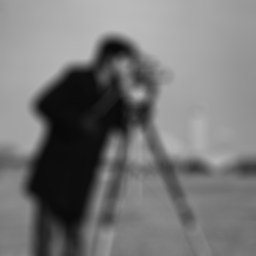
\includegraphics[scale=0.8]{lensblur17.png}

\includegraphics[scale=5]{kern_lensblur17.png}
\caption{Unschärfe durch Defokussierung mit einem Radius von 8 Pixel
synthetisch hergestellt, ortsinvariant; rechts: der zugehörige Kern, 5fach
vergrößert}%
\label{figure_lensblur}
\end{figure}

\begin{figure}[htbp]
\centering
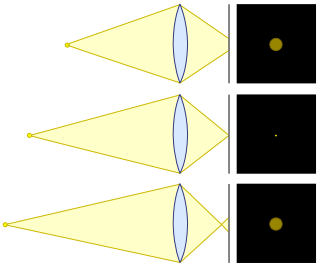
\includegraphics[scale=0.5]{Cirles_of_confusion_lens_diagram.png}%
\caption{Kern und Unschärfe. Illustration aus Wikipedia Commons
\cite{circleofconfusion}}%
\label{figure_confusion}
\end{figure}

\subsubsection{Allgemein dünn besetzter Kern}
Allgemein dünn besetzte Kerne weisen viele Pixel auf, dessen Grauwerte den Wert
Null haben. Die Gleichung \ref{eq:faltung1} zeigt, dass bei der Faltung jeweils
die Grauwerte der PSF als Faktor einfließen. Wenn nun viele Pixel der
Punktbildfunktion den Grauwert Null besitzen, können sie in der Berechnung
übersprungen werden. Die Abbildung \ref{figure_duenn} zeigt einen solchen Kern mit einem gefalteten Bild.

Solche Faltungskerne wirken anfänglich eher abstrakt, sie können aber praktische
Bedeutung haben. Wir stellen uns einen Kern mit Bewegungsunschärfe vor, dessen
Hauptrichtung diagonal verläuft. Das ist dann ein Kern, der nicht mit dem
1D-Boxfilter berechnet werden kann. Eine weitere Anwendung können Objektive mit
kodierter Blende sein. Dabei wird die Form der Blendenöffnung verändert
(\ref{figure_coded_apperture}). Der Vorteil einer solchen Blendenöffnung liegt
darin, dass man die Größe des Kerns leichter bestimmen kann. Die Tiefenschärfe
ändert sich ja mit dem Abstand des abgebildeten Objekts. Die Form der
Blendenöffnung wird so gewählt, dass sich das gefaltete Ergebnis abhängig von der Größe des Kerns
maximal ändert. Einen ähnlichen Ansatz verfolgt die Idee des kodierten Shutters
\cite{coded_shutter}. Hier wird die Belichtung nicht kontinuierlich 
durchgeführt, sondern in variablen Pulsen. Diese Methode kann besonders bei
periodischen Strukturen spezielle Vorteile bringen und die Dekonvolution stark
verbessern. Hier gilt dasselbe wie bei der Bewegungsunschärfe. Wenn die
Unschärfe in exakter horizontaler oder vertikaler Richtung verläuft kann die
übliche Faltung effizient verwendet werden. Wenn die Bewegungsrichtung jedoch
diagonal verläuft, kann ein Filter mit dünn besetzten Kernen uU. effizienter
sein.






\begin{figure}[htbp]
\centering
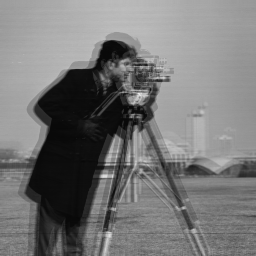
\includegraphics[scale=0.8]{out_krumm17.png}

\includegraphics[scale=5]{krumm17.png}
\caption{Unschärfe durch untypische PSF, rechts der passende Faltungskern
(vergrößert), wenig Pixel besetzt}%
\label{figure_duenn}
\end{figure}

\begin{figure}[htbp]
\centering
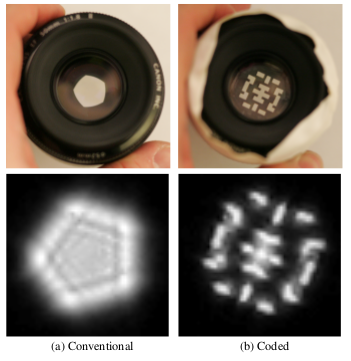
\includegraphics[scale=0.8]{coded_aperture.png}
\caption{coded aperture, entnommen aus \cite{coded_aperture}}%
\label{figure_coded_apperture}
\end{figure}

\begin{figure}[htbp]
\centering
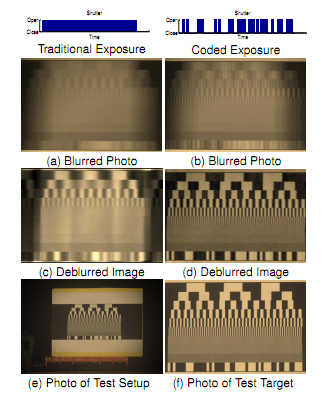
\includegraphics[scale=0.8]{coded_shutter.png}
\caption{coded shutter, entnommen aus \cite{coded_shutter}}%
\label{figure_coded_shutter}
\end{figure} 
\newpage












\subsection{Übliche Faltungsmethoden}\label{chp:faltungen}
Die Faltung mit den zuvor kennengelernten Faltungskerne werden idR. allgemein
mithilfe der Faltung im Orts- oder Fourierbereich durchgeführt. Wir kommen
zunächst zur Faltung im Ortsbereich.

\textbf{Ortsfaltung} Die Faltungsfunktion
(\ref{eq:faltung1}) wird im Diskreten zur folgenden Gleichung:

\begin{equation} \label{eq:faltungssumme}
%%(f*g)(x,y) =  \sum_{m=-K}^{K} \sum_{n=-K}^{K}{f[m,n] g[x-m,y-n]}
%%(f*g)(n) =  \sum_{m=0}^{N-1}{f[m] g[n-m]}
(f*h)[n] = \sum_{m=-k}^{k} {f[n-m] \cdot h[m]}
\end{equation}

Um ein Pixel des Ausgangsbildes zu erhalten müssen also die umliegenden Pixel des Eingangsbildes mit den Kernpixel
multipliziert werden. Das Eingangsbild besitzt $N$ Pixel und der Kern hat $K=2k$
Pixel. Für die Berechnung des vollen Bildes resultiert daraus
eine Laufzeit von $\mathcal O(N\cdot K)$. Sie ist also stark von der Kerngröße
abhängig. Die Abb.\ref{figure_IlluFaltung} schematisiert die
Berechnungsvorschrift. Der Einfachheit halber wurden hier die Indizes im
gerasterten Bildausschnitt von $-4$ bis $4$ nummeriert. 
 
\begin{figure}[htbp]
\centering
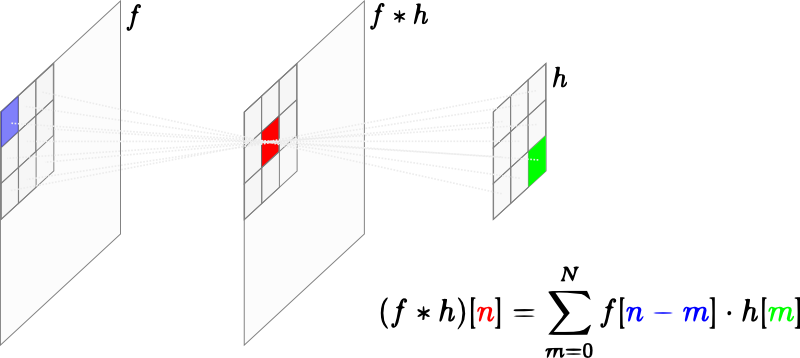
\includegraphics[scale=1.0]{faltung_illustration.png}
\caption{Illustration der Faltung im Ortsbereich}%
\label{figure_IlluFaltung}
\end{figure}

Häufig kommt ein
punktgespiegelter Kern zur Anwendung: $h^{*}(x) = h(-x)$. In diesem Fall
entspricht dann die Faltung der Korrelation: 

\begin{equation} \label{eq:korrelation}
(f*h^*)[n] = \sum_{m=-k}^{k} {f[n+m] \cdot h[m]}
\end{equation}
 
\textbf{Faltung im Fourierbereich}. Die Faltung im Frequenzbereich macht
sich das Faltungstheorem zu Nutze. Siehe dazu (\ref{eq:faltungssatz}). Dabei wird aus
einer Faltung im Ortsbereich eine Multiplikation im Fourierbereich. Die Laufzeit
wird dadurch besonders bei größeren Kernen wesentlich reduziert. Die Laufzeit
entspricht hier laut O-Notation dann $\mathcal O(N\log_2 (N))$, sie ist also von
der Kerngröße unabhängig.
\begin{equation} \label{eq:faltungssatz}
f(x) * h(x) \rightarrow F(u) \cdot H(u)  
\end{equation}
 
\textbf{Randbehandlung}. Bei der Faltung im Orts- und Fourierbereich kann es zu
Bereichs\-überschreitungen bei Arrayzugriffen kommen. Wir betrachten
zuerst die Faltung im Ortsbereich. Bereits wenn das erste Pixel des Ausgangsbild
berechnet werden soll muss laut Berechnungsvorschrift auf ein Eingangspixel zugegriffen werden, das es gar nicht gibt: 
\begin{equation} \label{eq:randbehandlung}
(f*h)[0] = \sum_{m=-k}^{k} {f[0-m] \cdot h[m]}
\end{equation}
Bei einer Kerngröße von $5$ muss das Pixel $f[0-5]$ des Eingangsbildes definiert
werden, da es ja nicht existiert. Dazu gibt es verschiedene Möglichkeiten. Man
kann dieses Randpixel als $0$ annehmen, oder auch mit einem anderen konstanten
Wert festlegen. Es bietet sich auch an die Randpixel über den Rand hinaus zu
spiegeln. Genauso ist es denkbar, dass man nicht auf das Pixel $f[0-5]$
zugreift, sondern auf das nächstgelegene: $f[0]$.

Nun betrachten wir die Faltung im Frequenzbereich. Die Fouriertransformation
impliziert eine periodische Fortsetzung des Signals. Bei der Implementation tritt
keine Bereichsüberschreitung bei Arrayzugriffen auf. Deshalb kann die
periodische Fortsetzung ohne Implementationsaufwand umgesetzt werden. Durch den
Rand entsteht dann jedoch auch ein unnatürlicher Frequenzgang, der dann bei der
Dekonvolution zu "`Ringing-Artefakten"' führen kann. Wenn diese Artefakte zu
stark werden, können mit weiterem Rechenaufwand andere Randbehandlungen
implementiert werde, wie zum Beispiel die Spiegelung am Bildrand.


\subsection{Dekonvolutionsalgorithmen}\label{chp:algoritmen}

\textbf{Inverse Filterung, Wienerfilter }\cite{wiener}. 
Mit dem Faltungssatz wurde gezeigt, dass die Faltung im Ortsbereich
zu einer Multiplikation im Frequenzbereich wird (\ref{eq:faltungssatz}).
Naheliegend scheint also diese Multiplikation durch eine Division mit dem
bekannten Faltungskern umzukehren:  $\hat u = \frac{\hat{f}(\omega)}
{\hat{h}(\omega)}$. Da aber der Faltungskern Nullstellen besitzen kann, enstehen
undefinierte Ergebnisse durch eine Division durch Null. Der inverse Filter ist
also praktisch nicht realisierbar. Häufig verwendet wird jedoch der
Wienerfilter:

\begin{equation} \label{eq:wiener}
\hat{u} = \frac{\hat{f}\cdot\bar{\hat{h}}} {|\hat{h}|^{2}+K}
\end{equation}

Dabei ist $\hat{f}$ das fouriertransformierte und unscharfe Eingangsbild. Das
geschärfte Ausgangsbild wird im Frequenzbereich mit $\hat{u}$ dargestellt und
der fouriertransformierte Faltungskern wird mit $\hat{h}$ ausgedrückt. Da diese
Größen also fouriertransformiert wurden, erfolgen die Rechenoperationen nun
im Komplexen. Die Division 
erfolgt jedoch mit einem reellen Divisor, dem quatratischen Betrag des
fouriertransformierten Faltungskerns $|h^*|^2$.
Dazu wird der Wert $K$ addiert. Dieser Wert wirkt als Regularisierer und
beseitigt das Problem der Nullstellen von $|\hat{h}|^{2}$. Die Multiplikation von
$\hat{f} \cdot \bar {\hat{h}}$ ist hingegen eine Rechenoperation mit Real- und
Imaginärteil und zwar mit dem komplex Konjugierten von $h^{*}$. Der Wienerfilter
kann mit $K$ justiert werden: Wenn ein großes $K$ gewählt wird, ist der
Schärfungseffekt gering. Wird ein kleines $K$ gewählt, so ist die Schärfung
besser. Allerdings nimmt dann auch das Rauschen zu. Der Wienerfilter ist eine
lineare Methode und wird durch die Fouriertransformation und komplexer
Multiplikation effizient implementiert. Der Einsatz des Wienerfilters ist durch
die Stärke des Rauschsignals begrenzt.


\textbf{Richardson-Lucy} \cite{richardson,lucy}
Ein häufig verwendeter iterativer Dekonvolutions\-algorithmus ist die Methode
von L. B. Lucy \cite{lucy} und William Hadley Richardson \cite{richardson}, nun als
RL bezeichnet:

\begin{equation} \label{eq:rl}
u^{k+1}= \left( h^* * \left( \frac{f}{u^{k}*h}\right) \right) \cdot{u^{k}}
\end{equation}

Mit der Berechnung von $u^{1}$ wird die Iteration gestartet und als Anfangswert
wird $u^{0} = f$ gewählt. Der Algorithmus erfodert die Division durch das
Zwischenergebnis $u^k*h$. Dabei wird also mit dem bekannten Faltungskern
gefaltet. Die zweite Faltung erfolgt dann mit dem punktgespiegelten Kern $h^*$,
die falls der Kern punktsymmetrisch sein sollte ($h^*(x) = h(-x)$), einer
Faltung mit dem Kern entspricht. Ein Wechsel in den Forierbereich ist hier nicht
erforderlich. Die Faltungen können im Orts- oder Frequenzbereich berechnet
werden. Der RL Algorithmus ist eine
Fixpunktpunktiteration.
Er verwendet eine Likelihood-Schätzung und basiert auch dem
Poisson-\-Rauschmodell.
Der Algorithmus erfordert als Parameter nur die Anzahl der Iterationen. 
RL erfordert positive Grauwerte des Eingangsbildes und
arbeitet während der Iteration auch positivitätserhaltent. Es zeigt sich ein semi-konvergentes Verhalten. 
Dabei wird das Rauschen verstärkt und führt nach einer Konvergenzphase der
Schärfe zur Divergenz hinsichtlich des Rauschverhaltens.
 


\textbf{Robust Regularisierter Richardson-Lucy} \cite{rrrl}
Der RL-Algorithmus wird nun mit folgendem Funktional in Bezug gebracht:
\begin{equation} \label{eq:functional1}
E_{f,h}[u]:=\int_\Omega \left (u*h-f-f \cdot \mathrm{ln} \frac{u*h}{f}  \right )\mathrm{d}x
\end{equation}
wobei es nun mit der Substitution $r_f(v):=v-f-f \cdot \mathrm{ln}(v/f)$
abgekürtzt geschrieben werden kann als:

\begin{equation} \label{eq:functional2}
E_{f,h}[u]:=\int_\Omega \Phi(r_f(u*h))+ \alpha \Psi (|\nabla|^2) \mathrm{d}x 
\end{equation}

Dabei sind $\Phi$ und $\Psi$ Straffunktionen und $\alpha$ ein Regularisierer,
der abhängig vom Rauschpegel zu wählen ist.

Schließlich läßt sich aus dem Funktional
(\ref{eq:functional2}) eine Euler-Lagrange Gleichung und eine weitere
Fixpunktiteration, ähnlich zu (\ref{eq:rl}) ableiten:


\begin{equation} \label{eq:rrrl}
u^{k+1} = \frac{(\Phi' (r_f(u^k *h))\frac{f}{u^k*h})*h^*+\alpha
[\mathrm{div}(\Psi'(|\nabla u^k|^2) \nabla u^k )]_+}{\Phi'
(r_f(u^k*h))*h^*-\alpha[\mathrm{div}(\Psi'(|\nabla u^k |^2)\nabla u^k)]_-}u^k
\end{equation}

wobei die Ausdrücke in den Klammern $[z]_\pm := \frac{1}{2}(z\pm |z|)$ sind.
Diese Gleichung ist also wieder eine Iteration und wird "`robust regularisierter
Richardson Lucy-Algorithmus"' genannt \cite{rrrl}. Er ermöglicht die
Dekonvolution bei gleichzeitiger Verwendung einer Regularisierung über die
Straffunktionen und dem Regularisierungsparameter $\alpha$.









 

\subsection{Ansatz für Optimierungen}
In \cite{rrrl} wurden bereits Möglichkeiten für eine schnelle Berechnung
vorgestellt. Dabei wurde die Faltung im Fourierbereich verwendet. Sie stellt das
Grundwerkzeug für eine effiziente Berechnung der Faltung dar. Die Schnelle
Fourier-Transformation ist sehr gut pa\-ral\-lelisier\-bar. In \cite{rrrl} wurde
auch eine Variante implementiert, die zuerst ein heruntergerechnetes Ergebnis als
Zwischenergebnis für die Iteration verwendet ("`course-to-fine"'-Ansatz).

In \cite{vimpaper} wurde der 1D-Boxfilter für die Vorwärtsfaltung
in RL und RRRL angewandt. Der 1D-Boxfilter \cite{mcdonnell} ist eine
Implementierung der Faltung mit einem ganz speziellen Faltungskern 
(wie bereits gezeigt im Kap. \ref{chp:einf_unschaerfe}).
Ebenso wurde im Paper \cite{vimpaper} der RRRL eingesetzt, wobei als Anfangswert
$u^0$ ein mit dem Wienerfilter vorberechnetes Bild zugeführt wurde.

Dass Faltungskerne separierbar sind und dadurch in ihrer Berechnung Speicher
sparen, wurde von Lehmann et at. gezeigt \cite{lehmann}. Dieser Ansatz wurde bei
der Implementation des separierten Boxfilters gewählt.

Wenn der Ansatz aus \cite{vimpaper} nun aufgegriffen wird und dabei weitere
Faltungsroutinen für spezielle Kernformen entwickelt werden, könnte uU. die 
Performance eines FFT
erreicht oder übertroffen werden. Eine mit SIMD ("`single
instruction on multiple data"') paral\-lelisierte Implementierung
wurde unter \cite{sse} vorgestellt. Hier wurde der SSE2-Befehlssatz verwendet.

Ein Auszug aus dem Profiler zeigt uns in Abb. \ref{figure_gprof} den
Rechenaufwand der Faltung am De\-konvolutions\-prozess eines RL-Algorithmus. 
Demnach verbaucht die Ortsfaltung über 90\% der gesamten
Berechnungszeit. Die Optimierung der Faltungsroutinen scheint also lohnend.

Wenn man ebenso bedenkt, dass bei der Iteration die Schärfung von Pixel zu Pixel
unterschiedlich und mit steigender Iterationszahl langsamer \cite{rrrl}
geschieht, kann auch die genaue Analyse der Konvergenz von konkreten
Eingangsbildern eine Beschleunigung bringen.



\begin{figure}[htbp]
\framebox[\textwidth] {
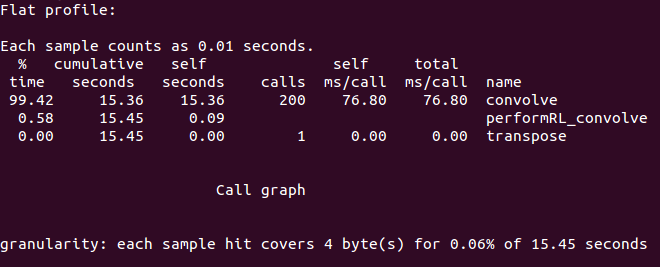
\includegraphics[scale=0.6]{gprof.png}}
\caption{Ausgabe von gprof zum RL mit Ortsfaltung}%
\label{figure_gprof}
\end{figure}
 
\newpage

\section{Zielsetzung}
Für die iterativen Dekonvolutionsalgorithmen im Abschnitt \ref{chp:algoritmen}
und die in Abschnitt \ref{chp:einf_unschaerfe} gezeigten Faltungskernen sollen
schnelle Verfahren entwickelt werden. In diesem Zusammenhang sollen zwei Wege
verfolgt werden: Die Optimierung der Faltungsoperation (siehe
Abschnitt \ref{chp:ziel1}) und die Optimierung hinsichtlich des
Konvergenzverhaltens einzelner Pixel (siehe Abschnitt \ref{chp:ziel2}).

\subsection{Filterdesign} \label{chp:ziel1}

In jeder Iteration ist die Faltung mit dem bekannten Kern (der
Punktbildfunktion) notwendig. Diese Faltung ist der mit Abstand aufwändigste Teil 
der Iteration und stellt somit den entscheidenden Schritt der Optimierung
dar. Dazu sollen die nun folgenden Faltungskerne näher untersucht werden:

\begin{itemize}
  \itemsep -1pt 
  \item 1D-Boxfilter (Abb. \ref{figure_motion})
  \item 2D-Boxfilter (Abb. \ref{figure_motion2d})
  \item Lensblur (Abb. \ref{figure_lensblur})
  \item allgemein dünn besetzte Kerne (Abb. \ref{figure_duenn})
\end{itemize}

Der 1D-Boxfilter wurde im Zusammenhang mit RL und RRRL bereits verwendet und
soll zum Vergleich zu den weiteren Filter herangezogen werden. Der 2D-Boxfilter
wurde als Faltungsroutine schon untersucht und eingesetzt, im Zusammenhang mit
iterativen Dekonvolutionsalgorithmen jedoch noch nicht. Er kann auf verschiedene
Arten implementiert werden. Etwa durch Hintereinanderausführen von zwei
1D-Boxfiltern oder durch die Vorberechnung eines kumulierten Grauwertbildes. 

Die Bedeutung des 2D-Boxfilters ist nicht so groß wie die der zwei folgenden:
Der Lensblurfilter modelliert wie bereits gezeigt (\ref{chp:einf_unschaerfe})
die Defokussierungsunschärfe. Mit einem besonders effizient implementierten
Lensblur-\-Filter kann ein iterativer Dekonvolutions\-algorithmus die
Defokussierungsunschärfe in Fotos schnell korrigieren. Der praktische Nutzen ist
demnach sehr hoch.

Die allgemein dünn besetzten Kerne bieten ebenso vielfältige
Einsatzmögklichkeiten. Wie in Kapitel \ref{chp:einf_unschaerfe} lassen sich mit
einem solchen Filter diagonale Bewegungsunschärfen effizient entfernen.

Zu den genannten Filtern soll die schnellste Implementierung gefunden werden und
die Rechenzeit abhängig von der Kerngröße ermittelt werden.


\subsection{Analyse des Konvergenzverhaltens} \label{chp:ziel2}
Mit steigender Iterations\-zahl nimmt die Schärfung zu und der Anteil
der Regularisierung sinkt \cite{rrrl}. Das wirkt sich negativ auf das
Rauschverhalten aus und gleichzeitig weiß man nicht genau, nach wievielen
Iterationen die gewünschte Schärfung eintritt. Ebenso ist anzunehmen,
dass sich die Grauwerte mancher Pixel stärker und schneller ändern.
Beispiels\-weise werden sich Pixel in der Nähe einer Kante anders verhalten, als
die Pixel in einer homogenen Umgebung. Pixel mit einer schwachen bzw. langsamen Grauwertänderung können in den darauf
folgenden Iterationen übersprungen werden, um Rechenzeit ein\-zusparen.
Gesucht ist ein Maß für die Konvergenz bei gleichbleibenden Ergebnissen.
Ob Rechenzeit gespart wird, ist zu evaluieren.


 
\newpage
%%%%%%%%%%%%%%%%%%%%%%%%%%%%%%%%%%%%%%%%%%%%%%%%%%%%%%%%%%%%%%%%%%%%%%
%%%%%%%%%%%%%%%%%%%%%%%%%%%%%%%%%%%%%%%%%%%%%%%%%%%%%%%%%%%%%%%%%%%%%%
 
\section{Methoden}
\subsection{Softwareumgebung}
Um eine effiziente, maschinennahe Implementierung zu ermöglichen wurde die
Sprache C verwendet. Auf objektorientierte Programmierung wurde verzichtet.
Durch die prozedurale Implementierung können unbeabsichtigte Aufrufe von
Konstruktoren, Überladungen und ähnlicher C++ Elemente vermieden werden und der
Fokus kann auf den effizienten Programmablauf gelegt werden. Ich folge dem
Sprachstandard ANSI C.

Zur Implementierung: Es liegen bereits sämtliche Routinen zur Ein- und
Ausgabe, sowie die Dekonvolutionsverfahren RL und RRRL vor. 
Die genannten Optimierungen (\ref{chp:ziel1} und \ref{chp:ziel2}) sollen implementiert
und evaluiert werden.

\subsubsection{System}
Als Betriebssystem wurde Ubuntu 11.10 mit 32 Bit gewählt. Alle Implementierungen
sind plattformunabhängig erfolgt. Also ist der Sourcecode ebenso unter Windows
lauffähig. Die einzige Ausnahme ist die Zeitmessung. Hier wurde eine
Linux-spezifische Systemfunktion verwendet.
\subsubsection{Compiler und Linker}
Es wurde GCC 4.6.1 gewählt. Der Compile- und Linkvorgang erfolgt in einem
Aufruf. Es musste somit kein Makefile verwendet werden.
Der Aufruf erfolgt folgendermaßen:
\begin{lstlisting} [caption={Kompileraufruf}]
 gcc ../main_rl.c ../pgmio.c ../functions.c -O2 -Wall -lm -o rl.out
\end{lstlisting}
\begin{itemize}
  \itemsep -1pt  
\item \textbf{main\_rl.c} stellt die main-Routine zur Verfügung. Hier werden die
Routinen zur Dateiein- und ausgabe sowie die Algorithmen aufgerufen
\item \textbf{pgmio.c} stellt die Dateiein- und ausgabe zur Verfügung
\item \textbf{functions.c} stellt alle Algorithmen zur Verfügung; darunter sind
die Dekonvolutions\-algorithmen, die FFT (Fast Fourier Transformation) und die
Faltungsroutinen;
\end{itemize}
Der Schalter "`-O2"' bewirkt die Optimierung mit Level 2 und faßt damit
verschiedene Compiler-Schalter zusammen \cite{gcc}.
In der Entwicklung kam zusätzlich Eclipse mit der Erweiterung CDT (C/C++
Development Tooling) zum Einsatz. Entsprechende Projectfiles liegen vor.

\textbf{Libraries:} Der Einsatz von externen Libraries sollte
möglichst vermieden werden. Eingebunden wurden die nun folgenden Headerfiles:
\begin{itemize} 
  \itemsep -1pt 
  \item stdlib.h
  \item	stdio.h
  \item	math.h
  \item sys/time.h spez. Linux-Zeitmessung
\end{itemize}
Eine einzige systemabhängige Funktion wurde verwendet:
Die Datei "`time.h"' musste für die Zeitmessung mit der Routine
"`gettimeofday()"' eingebunden werden. Wenn der Sourcecode unter einem anderen
System lauffähig gemacht werden soll, wird eine equivalente
Zeitmessung benötigt. Unter \cite{fastcode} sind verschiedene Varianten der
Zeitmessung aufgeführt. 
Außerdem kann für Windows eine Funktion aus
der WIN32 API und zwar die Routine "`GetSystemTime(..)"' unter Einbindung der
Headerdatei "`Winbase.h"' verwendet werden \cite{petzold}.


\subsubsection{Dateiformat}
Wir wollen die Bilder in einem verlustfreien Format einlesen und ausgeben.
Außerdem soll die Verwendung externer Libraries möglichst vermieden werden.
Dabei bietet sich das  Format "`Portable-Greymap"' an. Es stellt eine
kompressionsfreie und somit auch verlustfreie Dateienein- und -ausgabe für
RGB-Bilder als auch für Grauwertbilder zur Verfügung.


\textbf{pgm - portable greymap}
Die Spezifikation ist unter \cite{pgm} zu finden.
Das pgm-Format ermöglicht die Verarbeitung von 8-Bit-Grauwerten und 16-Bit. 
Die Daten können entweder als ASCII-Zeichen oder aber auch als Binärdaten
gespeichert werden. Wir implementieren die Speicherung im Binärformat und 8 Bit.
Im Listing \ref{lst:pgm} wird der relevante Codeauschnitt zu pgm - portable greymap 8bit gezeigt.

\begin{lstlisting} [float,caption={PGM Dateien einlesen und
schreiben},label=lst:pgm] 
...
// read 8bit values
int i;
for(i=0; i<size; i++){
  value = fgetc(fp);
  // check for error / EOF
  if((int)value == EOF){
     printf("\nError occured.);
     fclose(fp);
     return 0;
     }
     // save current pixel value in 1D array
     (*pixels)[i] = value;
}
...

 // write 8bit values
 for(i=0; i<size; i++){
	value = (*pixels)[i];
	// check if value is in correct range
	if(value < 0.0){
		c = 0;
	}
	else if(value > 255.0){
		c = 255;
	}
	else{
		c = (unsigned char) (value);
	}
	// write character
	fputc(c,fp);
}
...
\end{lstlisting}

\subsubsection{Datenorganisation und Pixelzugriff}
Wenn man überlegt, wie die Daten eines Bildes zu speichern sind, würde man
gleich auf ein zweidimensionales Array schließen, weil ein Bild ja auch
zweidimensionale Daten repräsentiert. Warum das idR. weniger
effizient ist als ein eindimensionales Array wird unter \cite{fastcode}
erläutert. Wenn ein Speicherblock für ein eindimensionales Array alloziert wird,
kann davon ausgegangen werden, dass ein zusammenhängender Block angelegt wird.
Da die Bildgrößen zur Laufzeit nicht bekannt sind, wird das System die
Speicherblöcke und Teile davon auf die verschiedenen Speicherstufen verschieben.
Wie diese Stufen meist aufgebaut sind, zeigt die Abb. \ref{figure_cache} aus dem
Artikel \cite{fastcode}.

\begin{figure}[htbp]
\centering
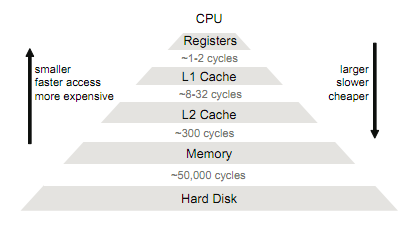
\includegraphics[scale=0.8]{cache.png}
\caption{Hier sind die Speicherhirachie mit den Zugriffszeiten schematisch
dargestellt. Die tatsächlichen Werte hängen von der verwendeten Hardware ab.
Die Abbildung stammt aus \cite{fastcode}.}
\label{figure_cache}
\end{figure}


Wie der Speicher konkret alloziert wurde, zeigt das Listing \ref{lst:array}.
Um darin auf ein einzelnes Pixel zuzugreifen, muss der Index anhand der Spalte
und Zeile rückgerechnet werden. Um eine effiziente Implementierung zu
gewährlisten, sollte ein Adresssprung auf eine andere Funktion möglichst
vermieden werden. Die Berechnung des Index sollte also möglichst "`inline"'
erfolgen. Dazu kann eine Funktion zur Indexberechnung entweder als
Inline-Funktion deklariert werden, oder die Berechnung direkt in der
Index-Klammer erfolgen. Bei der Optimierung wurde ein Makro eingeführt, das die
Berechnung am schnellsten ermöglicht: getPixelIndex(..) Siehe dazu Listing
\ref{lst:array}.


\textbf{int vs. float.} Die Verarbeitung von Gleitkommazahlen ist idR.
aufwendiger als das Rechnen mit Ganzzahlen. Deshalb stellt sich die Frage, ob
zur Bildberechnung ein Integer- oder Float-Format gewählt wird. Diese Frage läßt
sich leicht beantworten: Da die iterativen Dekonvolutionsalgorithmen die
Berechnung in Gleitkommazahlen vorraussetzen, kann nur ein Float-Typ verwendet
werden. Beim Speichern der Pgm-Datei wird eine Rundung ausgeführt.
Wir beschränken uns ja auf Bilder mit 8 Bit. Dennoch kann die Iteration nur mit
Gleitkommawerten berechnet werden, da sich ja viele Pixel um weniger als eine
Grauwertstufe pro Iteration ändern. Als durchgängiger Datentyp wurde also
"`Float"' gewählt.

 \begin{lstlisting} [float,caption={Speicherorganisation und
 Pixelzugriff},label=lst:array] Speicher alokieren:
Allokierung:
------------
float* g = (float*) malloc(unx*uny*sizeof(float));
// Die Groesse des erzeugten Bildes ist: unx*uny

Auf Pixel(10,0) zugreifen:
-------------------------
g[10] = ...
 
oder mit Makro:
#define getPixelIndex(row, col, nx, ny) (int)(((col) * (nx))+(row))
g[getPixelIndex(10,0,256,256)] = ...

// zusaetzliches Makro mit Bereichspruefung und Randbehandlung 'umbiegen'
#define getPixelIndexBend(row, col, nx, ny)\
	(int)(((col) < 0 ? \
	0 : ((col) >= (ny) ? \
	(ny)-1 : (col) ) * (nx)) + ((row) < 0 ? \
	0 : ((row) >= (nx) ? \
	(nx)-1 : (row))))

g[getPixelIndexBend(10,0,256,256)] = ...
\end{lstlisting}


\subsection{Verwendete Hardware}
Die Software wurde auf x86, also auf PC-Hardware implementiert. Zur Verfügung
stand eine Intel-CPU: $Intel^{\textregistered} Pentium^{\textregistered}
Processor P6100$ (3M Cache, 2.00 GHz). Sämtliche Optimierungen beziehen
sich auf diese CPU, welche über zwei Kerne verfügt. Implementiert wurden jedoch
keine parallelisierten Algorithmen, sodass nur ein Kern mit einem Thread
genutzt wurde.
 Hinsichtlich der Optimierung ist speziell das Speichermanagement relevant. Der
 Pentium P6100 verfügt über eine dynamische Cache-Architektur \cite{intel}. 
 Wenn eine andere CPU verwendet wird, sollte die Cache-Aufteilung
berücksichtigt werden. Unter Umständen ergeben sich nichtlineare
Laufzeitunterschiede durch eine Verlagerung mancher Speicherblöcke.



\begin{table}[htbp]
\begin{center}
\begin{tabular}{ | l | l |}
\hline
Feature			& Eigenschaft \\ \hline
No. of Cores			&	2 \\
No. of Threads		&	2 \\
Clockspeed	&	2 GHz \\
Intel Smart Cache		&	3 MB \\
Memory Types		&	DDR3-800/1066 \\
Max Memory			&	8 GB \\ \hline
\end{tabular}
\caption{CPU-Eckdaten Intel P6100\cite{intel}}
\label{tab:cpu}
\end{center}
\end{table}



\subsection{Filterdesign}\label{chp:filterdesign}
\subsubsection{1D Box}\label{chp:1dBox}
Der Boxfilter wurde von McDonnell bereits im Jahre 1981 beschrieben
\cite{mcdonnell}. Die Methode ermöglicht eine besonders effiziente
Implementierung der Faltung mit konstanten Grau\-werten: Die Bewegungsunschärfe
wurde in der Einleitung bereits beschrieben \ref{chp:einf_unschaerfe}.
Der 1D-Boxfilter wurde bereits im Zusammenhang
mit Dekonvolutionsalgorithmen untersucht: \cite{vimpaper}.
Die Methode kann folgendermaßen zusammengefasst werden:
Alle Pixel des Boxfilter-Kerns haben den selben Grauwert. Jedes erste Pixel in
einer Zeile, bzw. Spalte wird normal summiert (die Komplexität sit linear zur
Kerngröße und zum Eingangsbild). Durch die Größe des Boxfilters (bei einem 1D
Boxfilter sind das $1 \ast k$ oder $k \ast 1$ Pixel) ergibt sich ein gleitendes
Fenster.
Die Summe dieses gleitenden Fensters kann schnell ermittelt werden: Wenn das
Fenster um ein Pixel weiterverschoben wird, muss nur das überlappende Pixel zur
Summe des vorhergehenden Pixels ($n-1$) addiert werden (in der Abb.
\ref{figure_box} mit "`$+$"' markiert).
Das überlappende Pixel an der auslaufenden Kernseite wird subtrahiert.
(in der Abb. mit \ref{figure_box} mit "`$-$"' markiert)
Die Komplexität des Boxfilters in 1D beträgt: $\mathcal O(N+2K)$, Wenn $N$ die
Länge einer Zeile, bzw. einer Spalte ist und $K$ die Länge des Kerns. Das
bedeutet, dass sich die Laufzeit linear zur Größe des Eingangsbildes verhält.
  
\begin{figure}[htbp]
\centering
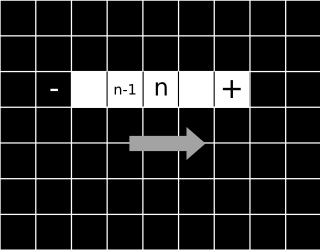
\includegraphics[scale=2.0]{Box1Di.png}
\caption{Illustration des 1D-Boxfilters}
\label{figure_box}
\end{figure}

\begin{lstlisting}[float,caption={Codeauschnitt 1D Box}]

	for(x=0;x<nx;++x) {

		// calc the first valid sum of current row
		for(kerny=-halflengthm;kerny<=halflengthp;++kerny) {
			   sum += upixel[getPixelIndexBend(x, kerny,nx,ny)];
		}

		// normalize the first pixel
		vpixel[getPixelIndexBend(x,0, nx, ny)] = sum * length_inv;

		// calc the following pixels just with adding 
		// the next and subtracting the previous
		for(y=1;y<ny;++y) {

			// add the pixel next to the kernel
			sum += upixel[getPixelIndexBend(x,(int)y+(halflengthp),nx,ny)];
				
			// subtract one pixel before the kernelmask
			sum -= upixel[getPixelIndexBend(x,(int)y-(halflengthm)-1,nx,ny)];
			
			// normalize
			vpixel[getPixelIndexBend(x,y,nx,ny)] = sum * length_inv;

		}
		sum = 0;        // set the running sum to zero for the next column
	}
}
\end{lstlisting}
 

\newpage

\subsubsection{2D Box}
Der Boxfilter mit einem Kern von $m \ast n$ Pixeln kann wie der 1D-Boxfilter
effizient implementiert werden. Implementiert wurden der 2D-Boxfilter als
separierter 1D-Boxfilter, nicht separierter 2D-Filter und kumulativer
Boxfilter.\\



\begin{verbatim}
\end{verbatim}


\begin{figure}[htbp]
\centering
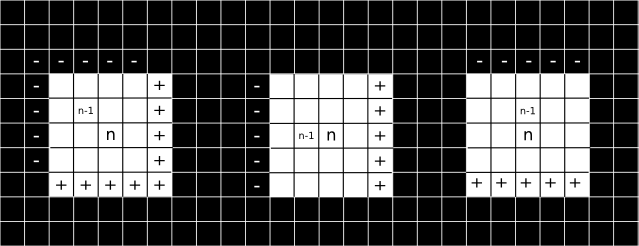
\includegraphics[scale=1.5]{Box2D.png}%
\caption{Illustration des 2D-Boxfilters}%
\label{figure_ill_box2d}
\end{figure}

\textbf{Nichtseparierter 2D-Boxfilter (zeilenweise)} 
Der Boxfilter kann für jedes Pixel zeilen- oder spaltenweise berechnet
werden. Wir behandeln das zeilenweise Vorgehen. Dazu wird erst das Pixel(0,0)
voll berechnet. Voll berechnet bedeutet folgendes: Alle Grauwerte der Pixel
in der Umgebung, die vom Kern aufgespannt wird, werden summiert. Danach wird die
erste Spalte berechnet: Dazu gibt es zwei Möglichkeiten. Entweder wird die
Spalte über ein gleitendes Fenster berechnet, oder die Berechnung erfolgt gleich
wobei Pixel(0,0). Implementiert wurde die zweite Variante. Wenn das Bild eine
Größe von $nx \cdot ny$ hat, haben wir nun $ny$-Pixel berechnet. Nun werden von
der ersten Spalte ausgehend alle anderen Pixel zeilenweise berechnet. Diese
Summation funktioniert nun über ein gleitendes Fenster. Es muss also jeweils
nur das rechte Randpixel des aktuellen Fensters addiert und das linke Randpixel
subtrahiert werden. Das zeigt die Abb. \ref{figure_ill_box2d}. Der Pseudocode
fasst den Ablauf zusammen: Listing \ref{lst:notsep}.

 
\begin{lstlisting} [caption={Pseudocode nicht separierter Boxfilter},label=lst:notsep] 
- Summe von Pixel(0,0) bilden
- Spalte(0) berechnen
- jede Zeile ausgehend von Pixel(0,n) berechnen
\end{lstlisting}



\textbf{Separierter 2D Boxfilter.} 
Der 2D-Boxfilter ist separierbar. So kann die
Faltung in zwei Schritten berechnet werden: $v = \left ( u \otimes h_{1} \right
) \otimes h_{2},dim(h_{1})=m\cdot1,dim(h_{2})=1\cdotn$.
Das heißt also, dass ein Boxfilter mit der Kerngröße $hx \cdot hy$ mit einem
1D-Boxfilter berechnet werden kann: Erst ein horizontaler 1D-Boxfilter mit der
Kernlänge $hx$ und anschließend ein vertikaler 1D-Boxfilter mit der Kernlänge
$hy$. Der Code vom 1D-Boxfilter wird somit wiederverwendet und benötigt keine
zusätzliche Implementation. Die Separierbarkeit von Faltungskernen wurde in
\cite{lehmann} diskutiert.




\begin{verbatim}
\end{verbatim}

 


\textbf{Kumulierter 2D Boxfilter}.
Aus einem Bild mit m*n Pixeln kann ein Bild mit den kumulierten Grauwerten
gebildet werden. Dabei entspricht der Grauwert des Pixels(k,l) der Summe aller
Pixelgrauwerte der Fläche eines Rechtecks, welches aufgespannt wird durch die
Eckpunkte Pixel(0,0) und Pixel(k,l).
Das kumulierte Bild kann wie in Abb. \ref{figure_kumuliert} berechnet werden:
Dabei werden die Pixelgrauwerte der ersten Zeile und der ersten Spalte
aufsummiert. Alle weitere Summen werden daraus errechnet und zwar nach der
Vorschrift, die im Listing \ref{lstlisting:cumulate} ersichtlich ist.
Ähnlich funktioniert der darauffolgende Filter:
Allerdings soll nun nicht die Summe des aufspannenden Rechtecks über dem Pixel,
sondern die Grauwertsumme der aufgespannten Kernfläche ermittelt werden.  

\begin{figure}[htbp]
\makebox[\textwidth] {
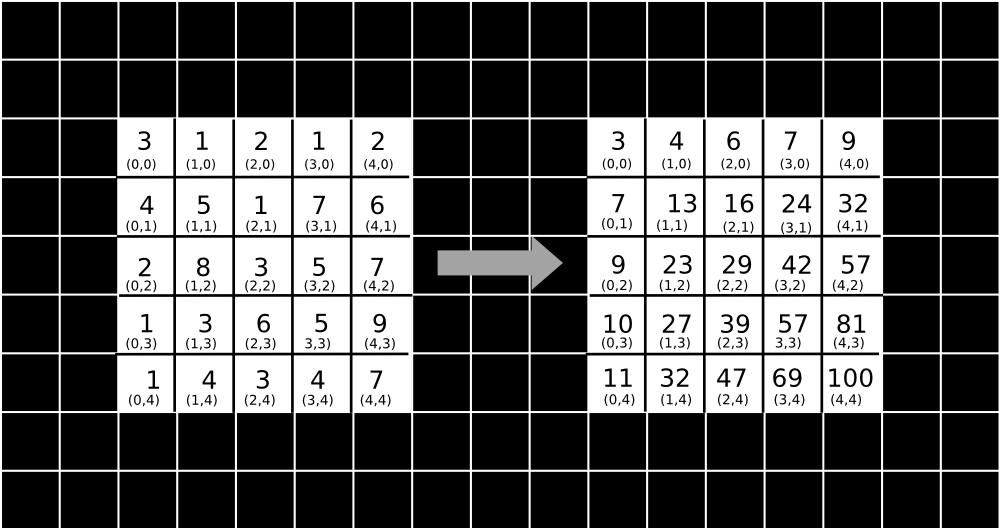
\includegraphics[scale=3.0]{BoxCumu.png}}
\caption{kumulierte Grauwerte}%
\label{figure_kumuliert}
\end{figure}


\begin{lstlisting} [float,caption={Pseudocode kumuliertes Grauwertbild},
label=lstlisting:cumulate]
- berechne erste Zeile:
	 von links nach rechts v(n,0) = v(n-1,0) + u(n,0)
	 
- berechne erste Spalte:
	 von oben nach unten v(0,n) = v(0,n-1) + u(0,n)
	
- jedes weitere Pixel:
von k=1 bis k=unx
	von l=1 bis l=uny 
		v(k,l) = v(k,l-1) + v(k-1,l) - v(k-1,l-1) + u(k,l)
\end{lstlisting}


\begin{lstlisting} [float,caption={Pseudocode kumulierter Boxfilter},
label=lstlisting:cumuBox]
von k=0 bis k=unx
	von l=0 bis l=uny 
		v(k,l) = 	u(k+hnx,l+hny) - u(k+hnx,l-hny-1) - u(k-hnx-1,l+hny) +
					u(k-hnx-1,l-hny-1)
\end{lstlisting}


Das entstandene Bild hat dann einen Wertebereich von 
$0 \ldots (g_{max} \cdot m \cdot n)$. Der Datentyp des kumulierten Bildes muss
demnach den auftretenden Wertebereich abbilden können. Bei einer verarbeiteten Bildgröße ist
das konkret: $256 \cdot 256 \cdot 256 = 2^{8} \cdot 2^{8} \cdot 2^{8} = 2^{24}$.
Single-Float Zahlen habe laut IEEE Standard 754-2008 eine Datenbreite von 32
Bit. Es werden 8 Bit für den Exponenten verwendet und 23 Bit für die Mantisse.
Da wir aber eine Genauigkeit von 24 Bit genötigen, ist streng
genommen der Datentyp "`Float-Double"' notwendig. 

Unser Datenarray für das kumulierte Grauwertbild muss demnach definiert
werden, als: $double* meinKumuliertesBild;$. Bei den implementierten
Zeitmessungen wurde jedoch ein Single-Float-Typ verwendet (da das Eingabebild
eine mittlere Helligkeit aufweist, ist auch kein Werteüberlauf passiert).



\begin{verbatim}
\end{verbatim}


\subsubsection{Lensblur, generischer Boxfilter}

\begin{figure}[htbp]
\makebox[\textwidth] { 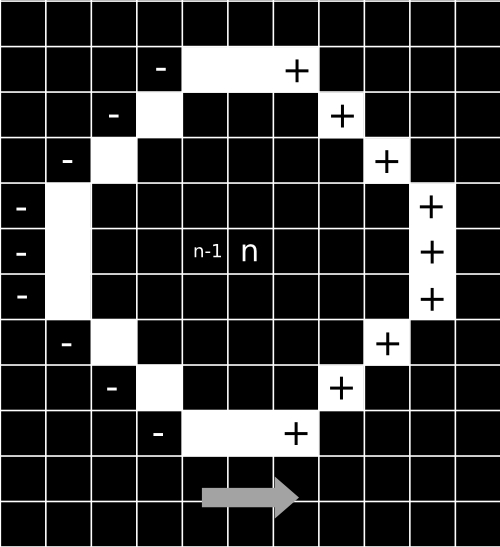
\includegraphics[scale=2.0]{lensblur_box.png} }
\caption{schneller Lensblur, Kern: Bresenham r=4px}
\label{figure_lensblur_box}
\end{figure}

\begin{figure}[htbp]
\makebox[\textwidth] { 
\includegraphics[scale=5.0]{bresenham.png} }
\caption{jeweils 3er Gruppen für den Lensblur Filter;
 mit ImageJ erzeugt, Bresenham mit einem Durchmesser von 9px, 11px und 17px,
 das entspricht einem Radius von 4px, 5px und 8 px}
\label{figure_bresenham}
\end{figure}

Die Abbildung \ref{figure_lensblur_box} illustriert die Methode, die in
Listing \ref{lst:genericBox} kurz beschrieben ist. Zu dem Algorithmus führen
zwei Ansätze, die zum Teil bereits vorgestellt wurden. Der nun vorgestellte
Faltungsalgorithmus wird aus drei einzelnen Teilen zusammengestellt und
ermöglicht eine effiziente Berechnug des Lensblur. Wenn der zu faltende Kern
über konstante Grauwerte verfügt und alle Pixel in einer Zeile zusammenhängen,
kann der Algorithmus verwendet werden. Die Details zeigen die folgenden zwei
Ansätze.
\\

 \begin{lstlisting} [float,caption={Pseudocode generischer
 Boxfilter},label=lst:genericBox]

 berechne erste Spalte: 
 	- Falte mit jedem Pixel des Kreises: 
 	  (256*58 Instruktionen)
 
 berechne alle anderen Pixel:	
 	- schiebe das laufende Fenster 
 	  um ein Pixel nach rechts: 
 	  (255*256*16 Instruktionen)
 	- normalisiere das aktuelle Pixel: 
 	  (255*256 Instruktionen)
 
 \end{lstlisting}

\textbf{Erster Optimierungsansatz}: Wenn wir den Kreis mit der Ortsfaltung
berechnen, sind $m \cdot n \cdot d \cdot d$ Gleitkomma-Multiplikationen
notwendig.
Dabei hat der Kern eine Größe von $d \cdot d$ Pixeln. Es wird jedes Pixel des
Eingangsbildes mit jedem Pixel des Kerns gefaltet. Wir beschränken uns auf die besetzten Pixel,
dh. auf die Pixel mit einem Grauwert größer als Null. Das führt uns auch schon zur
Methode des nächsten Kapitel: Listenfilter \ref{chp:listFilter}. Bei einem Kreis
können wir uns also auf die besetzten Pixel beschränken, was einer Kreis\-fläche
entspricht. Wir beschränken die Anzahl der Gleitkomma-Multiplikationen somit auf
$r^{2}\cdot \pi \cdot m \cdot n$. Ein Beispiel: Bei einem Faltungskern mit einem
Durchmesser und einem Eingangsbild von $256^{2}px$ sind nicht $256^{2}
\cdot 17^{2}$ notwendig, sondern nur mehr $256^{2} \cdot 8.5^{2} \cdot \pi$. Das
entspricht einer Optimierung um einen Faktor $8.5^{2} \cdot \pi / 17^{2}
\approx 227/289 \approx 0.78 $. Wir sparen hier also etwa 20 Prozent ein. 
Allerding steht dem ein Overhead für die algorithmische Umsetzung der
Pixelauswahl gegenüber.

\textbf{Zweiter Optimierungsansatz}: Jede Zeile des Kerns besteht aus
zusammenhängenden Pixeln. Es ist also möglich hier den Ansatz des Boxfilter 
anzuwenden: Wir berechenen das erste Pixel jeder Zeile und schieben wieder ein
"`sliding-window"' nach rechts, wobei die laufende Summe mit den überlappenden
Stellen berechnet werden kann. Siehe dazu Abbildung \ref{figure_lensblur_box}.
Die Summe aller Grauwerte im Kreis kann gebildet werden durch Hinzufügen der
mit "`+"' markierten Pixel und durch Abziehen der mit "`-"' markierten Pixel. Da die
Grauwerte aller Pixel des Kreises gleich sind, brauchen wir außerdem nur einmal
pro Eingangspixel normalisieren. Dazu ist eine Gleitkommamultiplikation nötig,
während die laufenden Summen ohne Multiplikation auskommen.\\
\textbf{Ansätze kombinieren:} Wir können die beiden Ansätze gleichzeitig
anwenden und kommen zu folgender Optimierung: Bei einem Kern mit Radius 4 und einem
Eingangsbild mit $256 \cdot 256$px brauchen wir theoretisch folgende
Rechenschritte (siehe Listing \ref{lst:genericBox}):
\\
Die Kreisfläche beträgt 57 Pixel (siehe Abb. \ref{figure_lensblur_box}).
Die erste Spalte müssen wir mit jedem Pixel des Kreises falten: $256 \cdot 57$
Additionen, 256-mal normalisieren (Multiplikation notwendig). Danach laufende
Summe für jedes Pixel nach der ersten Spalte berechnen: $255 \cdot 256 \cdot 16$
und normalisieren: $256^{2}$ mal. Macht also in Summe: $256 \cdot 58+255
\cdot 256 \cdot 17 = 1124608$ Instruktionen, während für die volle Ortsfaltung
$256^{2} \cdot 17^{2} = 18939904$ nötig sind. Das entspricht weniger als 6
Prozent.\\
Demnach lassen sich also 94\% der Laufzeit einsparen. Wieviel es dann im
praktischen Falle sind, werden die Ergebnisse im Kapitel
\ref{chp:mess_faltungen} zeigen.
 



\textbf{Vom Lensblur zum generischen Boxfilter}. Wie in Abb.
\ref{figure_lensblur_box} können wir mit dieser Methode einen Lensblur
berechnen. Es ist aber gleichzeitig möglich, mit dem Algorithmus in Listing
\ref{lst:genericBox} weitere Kerne abzubilden. Einzige Voraussetzung: Die Pixel
müssen konstant und in jeder Zeile zusammenhängend sein. Die Abbildung
\ref{figure_genBox} zeigt eine Auswahl an möglichen Kernen.


\begin{figure}[htbp]
\makebox[\textwidth] { 
\includegraphics[scale=5.0]{krumme_kerne.png} }
\caption{verschiedene Kerne für den generischen Boxfilter}
\label{figure_genBox}
\end{figure}
 

\subsubsection{Listenfilter, allgemein dünn besetzte
Kerne}\label{chp:listFilter}
Bereits beim Lensblur-Filter des vorigen Kapitels wurde der Optimierungsansatz
aufgegriffen: Wir beschränken uns auf jene Pixel, dessen Grauwert nicht Null
ist. Der Kern besteht anfänglich aus n Pixeln. Diese Pixel haben jeweils einen
Grauwert: $h(x)$. In der Implementation wird das in einem Array abgebildet
(siehe Listing \ref{lst:listData}). Aus diesen n Pixel werden nun k Pixel, dessen
Grauwert größer Null ist: $h(x) > 0$. Diese Pixel werden in drei Komponenten
abgebildet:
Einer x-Komponente, einer y-Komponente und einer Grauwert-Komponente. Diese
Komponenten werden jeweils als Arrays implementiert. Eine Übersicht der neuen
Datenstruktur bietet das Listing \ref{lst:listData}. \\
Während vorher bei der Ortsfaltung jedes Pixel des Eingangsbild mit allen
Kernpixeln gefaltet wurden (also multipliziert), kann nun eine
3-Komponenten-Liste durchgearbeitet werden. Der Vorteil zeigt sich, wenn viele
Pixel des Kernes nicht besetzt (gleich Null) sind.
Der Listenfilter wurde noch in einer Variante implementiert, die alle Grauwerte
des Kerns als konstant annimmt. Das Array mit den Grauwerten fällt dann weg und
aus einer Multiplikation mit den Kernpixeln wird eine Addition. Diese Variante
wird in der Folge als "`Listenfilter konstant"' bezeichnet.

 \begin{lstlisting} [float,caption={Datenformat des
 Listfilter},label=lst:listData] 
ALTES DATENFORMAT:
- Floatarray. zb: float h[100];
- Inhalt: h = {1.2, 3.5, 90.2, 77.2, 66.1, ...};
- Zugriff: 
h[10]	// 10tes Pixel
oder h[getPixelIndex(10,0,nx,ny)]	// 10tes Pixel der ersten Zeile

NEUES DATENFORMAT:
- drei Floatarrays mit x,y,g
zb:
int x[100];
int y[100];
float g[100];
- Inhalt:
x = {1, 2, 3, 5, 6, 7, ...}; // Liste der x-Koordinaten, 4tes Pixel=0
y = {0, 0, 0, 0, 0, 0, ...}; // Liste der y-Koordinaten
g = {1.2 , 10.5, 90.3, 37.4, 63.4, 72.1, ...}; // enthaelt Grauwerte!=0
- Zugriff:
g[10]	// 10tes besetzes Pixel
bzw:
for(i=0;i<listsize;i++) { if(x==10 && y==0) nehme Wert von g[...]}	
// zur Suche des 10ten Pixel muss die
Liste durchsucht werden!

 \end{lstlisting}


\subsubsection{Optimierung durch Paralellisierung: SIMD}\label{chp:simd}
Wie in der Einleitung bereits erwähnt, kann die Optimierung sehr
hardwarespezifisch erfolgen. In diesem Fall muss aber eine konkrete
Hardwareplattform zu Grunde gelegt werden. In dieser Arbeit konzentrieren wir
uns primär auf die nicht hardwarespezifische Optimierung. Ergänzend soll hier
jedoch noch eine einfach zu implementierende Variante gezeigt werden: Der
verwendete Comnpiler GCC bietet fertige Funktionen zur Verarbeitung mehrerer
Datenblöcken in einem Rechenschritt \cite{gcc}. Als Überbegriff ist wird hier
"`SIMD"' verwendet: "`single instruction, multiple data"'. SSE ist eine solche
Technologie und ist auf der x86-Plattform weit verbreitet. GCC stellt dafür die
"`x86 build-in functions"' zur Verfügung. Sobald der Compilerschalter "`-msse"'
in der Kommandozeile übergeben wird, sind weitere Funktionen verfügbar. Das
Listing \ref{lst:sse} zeigt die verwendeten Routinen.

Da die Optimierung jedoch auf der parallelen Multiplikation von Eingangsbild und
Kern in 4er Gruppen basiert, müssen diese Bilder jeweils in Vierergruppen
aligniert sein. Das bedeutet, dass die Länge des berechneten Vektors (Bildes)
ein vielfaches von 4 sein sollte.
 Unser Eingangsbild mit 256 mal 256 Pixeln ist bereits 4-aligned.
Jedoch können wir nur mit einem Kern rechnen, der ebenfalls 4-aligned ist. 

Spezielle Kernformen, wie zuvor gezeigt, können durch Parallelisierung leider
nicht weiter beschleunigt werden. Näheres dazu in der Diskussion.


\begin{lstlisting}[float,caption={verwendete x86
build-in-SSE-Erweiterungen},label=lst:sse] ...
for(kerny=0;kerny<hny;kerny++) {
	for(kernx=0;kernx<hnx-3;kernx=kernx+4) {
		
		uvec = __builtin_ia32_loadups(...); // load groups of four floats
		hvec = __builtin_ia32_loadups(...); // load groups of four floats
		// Multiply and Add the groups of four floats
		acc = __builtin_ia32_addps(acc, __builtin_ia32_mulps(uvec, hvec));
 
...
\end{lstlisting}
 


\subsection{Analyse des Konvergenzverhaltens}\label{chp:methodik_konvergenz} 
Wie unter \ref{chp:ziel2} bereits erwähnt wurde, nimmt die Schärfe des Bildes
mit steigender Iterations\-zahl zu. Der Begriff der Schärfe ist nicht klar zu
definieren. Wenn die Dekonvolution die Darstellung eines Fotos visuell
verbessern soll, ist es schwierig eine Maßzahl für diese subjektive Eigenschaft
zu finden. Daher verwenden wir einen praktischen Ansatz und iterieren so lange,
bis das Ergebnis visuell ausreichend verbessert wurde. Zunächst soll die Konvergenz
der Schärfe näher betrachtet werden. Da wir für die Schärfe keine Maßzahl
verwenden, betrachten wir einfach den Grauwertverlauf eines Pixels während der
Iteration. Wenn wir also ein Pixel isoliert betrachten lassen sich verschiedene
Maßzahlen ableiten. Wir betrachten nun die Grauwertvarianz und die
Grauwertdifferenz.


\textbf{Betrachtung der Varianz.} 
Die Abbildung \ref{figure_konver_altes_bild}
zeigt die Varianz als Grauwertbild. Auf ein Eingangsbild mit einem Lensblur von
17$px$ Durchmesser wurde der Robust Regularisierte Richardson-Lucy Algorithmus
angewandt. Die dunklen Stellen weisen auf eine starke Änderung während der
Iteration hin. Es fällt also auf, dass es viele Bereiche gibt, in denen die
Grauwertänderung nach der gesamten Berechnung nur gering ist. 

Mit Hilfe des Verschiebungssatzes kann die Varianz aus den Zwischenergebnissen
jeder Iteration berechnet werden:
 
\begin{equation} \label{eq:verschiebungssatz}
\sum_{i=1}^{n} (x_i - \overline{x})^2 = \left(  \sum_{i=1}^{n} x_i^2 \right ) -
\frac{1}{n} \left ( \sum_{i=1}^{n} x_i \right ) ^2
\end{equation}

Die Abbildung \ref{figure_konv_histogramm} stellt die Verteilung der
Standardabweichung dar.
Gezeigt wird die Werte nach 5, 50 und 100 Iteration bei Berechnung mittels
RL-Algorithmus. Nach 100 Iterationen nehmen Standardabweichung und Varianz zu.


\begin{figure}[htbp]
\framebox[\textwidth] { 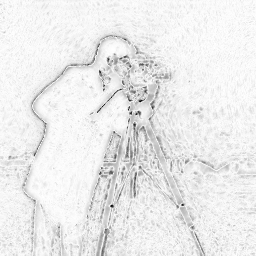
\includegraphics[scale=1.0]{konvergenz_std.png} }
\caption{Varianz bei RRRL, 0.000001, 0.1, 1000 Iterationen, invertierte
Darstellung}%
\label{figure_konver_altes_bild}
\end{figure}


\begin{figure}[htbp]
\makebox[\textwidth] {
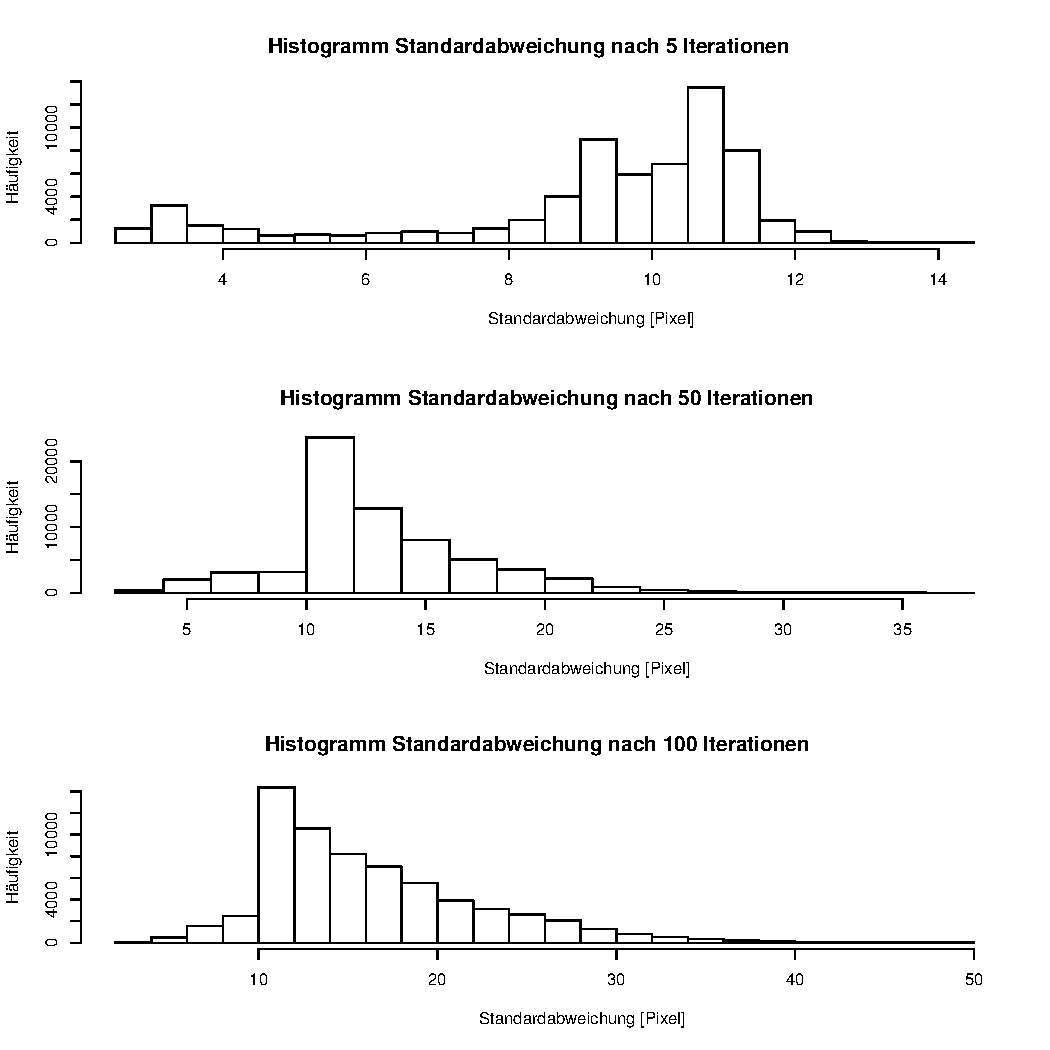
\includegraphics[scale=1.0]{histogramm_std_konvergenz.pdf} }
\caption{RL bei einem Lensblur von 17px, mit 5, 50 und 100 Iterationen.
Standardabweichungen der Grauwerte eines jeden Pixels}%
\label{figure_konv_histogramm}
\end{figure}
 
 
 
\textbf{Grauwertänderung von einer Iteration zur nächsten.}
Nun wurde einfach die Differenz $|u_k-u_{k-1}|$ gebildet und ausgewertet. Im
Diagramm der Abbildung \ref{figure_konv_verhalten} sieht man, dass nach der
ersten Iteration besonders starke Änderungen auftreten. Wenige Pixel ändern sich
innhalb einer Iteration um bis zu 20 Grauwerte. Weniger stark sind die
Änderungen nach der zehnten Iteration. Nach 50 Iterationen ändern sich die Pixel
schließlich um weniger als einen Grauwert pro Iteration. 

 \begin{figure}[htbp]
\makebox[\textwidth] {
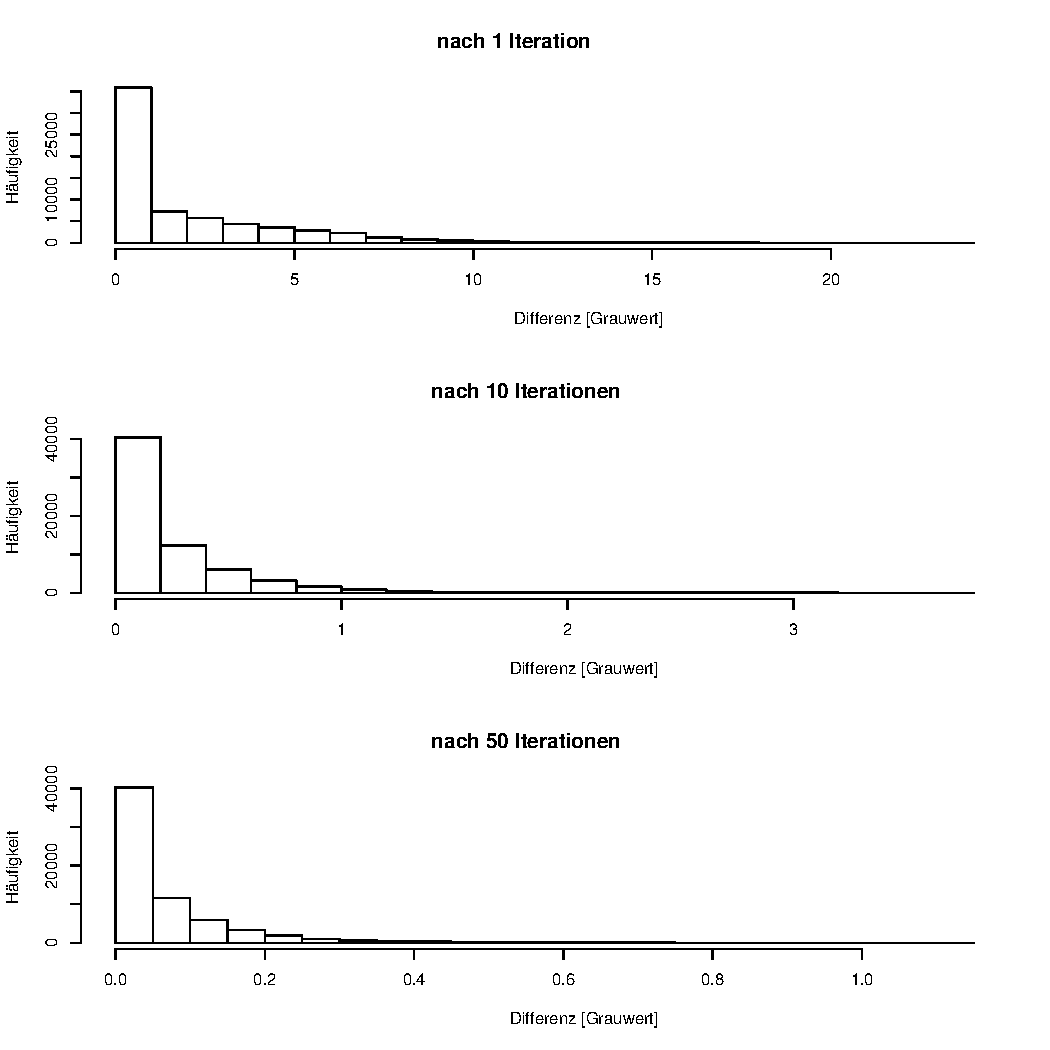
\includegraphics[scale=1.0]{Konvergenzverhalten.pdf} }
\caption{Grauwertänderung von einer Iteration zur nächsten;}%
\label{figure_konv_verhalten}
\end{figure}



\textbf{Optimierung}.
Es wurden mit der Varianz und mit der Grauwertdifferenz zwei Maßzahlen gefunden.
Nun soll anhand dieser Zahlen eine Optimierung entwickelt werden. Die Idee ist
folgende: Jene Pixel, die sich nur schwach ändern, werden auch nicht berechnet
und sparen dadurch Rechenzeit. Um dies zu ermöglichen, musste der Programmablauf
des Dekonvolutionsalgorithmus und der Faltung angepasst werden. Die Abbildung
\ref{figure_konverg_ablauf} schematisiert die Anpassung am RL-Algorithmus: Wenn
man einzelne Pixel in der Faltungsroutine ausläßt, muss ein Ersatzwert für die
darauf folgende Faltung und Iteration zugewiesen werden. Die roten Linien sollen
die Auswirkung auf die darauf folgenden Berechnungen zeigen. Das graue Pixel
wurde hier nicht gefaltet. Die Lösung ist folgende: Nach jeder Faltung wird das
Zwischenergebnis eines jeden Pixels gespeichert. Wird ein Pixel in der
aktuellen Iteration ausgelassen (nicht gefaltet), kann dessen Wert für die
darauffolgenden Berechnungen aus dem Zwischenspeicher der vorhergehenden
Iteration genommen werden. Im Programmablauf der Faltung muss eine
$if$-Abfrage hinzugefügt werden. Sie prüft, ob die Änderung des jeweiligen
Pixels für eine Bearbeitung ausreicht. Folgende Faltungsroutinen können mit
dieser Methode angewendet werden: die Ortsfaltung und der Listenfilter. Diese
zwei Routinen arbeiten Pixel für Pixel ab. Die Faltung im Fourierbereich
scheidet für diese Optimierung aus, da alle Pixel in den Frequenzbereich
zusammen transformiert werden müssen, um die Faltung durchzuführen. Die zuvor
gezeigten Boxfilter (1D-Boxfilter, 2D-Boxfilter, generischer Boxfilter oder
Lensblur) können mit dieser Optimierung ebenso nicht verwendet werden, da ihre
Berechnung auf dem Konzept der "`gleitenden"' Summen beruht und das Ausnehmen
einzelner Pixel so nicht möglich ist. Eine gemeinsame Optimierung mit dem
Listenfilter bietet sich jedoch an. Der Listenfilter hat die Eigenschaft, dass
er nur die besetzten Pixel berechnet. Wenn also ein dünn besetzter Kern mit
dieser "`konvergenz-optimierten"' Methode berechnet wird, sind zusätzliche
Einsparungen in der Rechenzeit möglich.


 
\begin{figure}[htbp]
\makebox[\textwidth] { 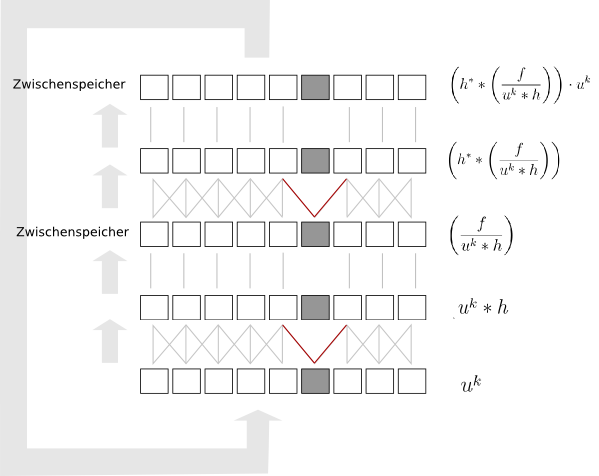
\includegraphics[scale=1.0]{ablaufRLOpti.png} }
\caption{Ablaufdiagramm der optimierten Version}%
\label{figure_konverg_ablauf}
\end{figure}

%%%%%%%%%%%%%%%%%%%%%%%%%%%%%%%%%%%%%%%%%%%%%%%%%%%%%%%%%%%%%%%%%%%%%
\newpage
\section{Ergebnisse}
\subsection{Messergebnisse Faltungsoptimierung}\label{chp:mess_faltungen}

Das Ziel der optimierten Faltungsroutinen, ist dass die Rechenzeit bei
gleichbleibender Qualität minimiert wird. Kurze Rechenzeit bei
gleichbleibendem Ergebnis wird nun als gute Performance bezeichnet.

\subsubsection{Qualitative Betrachtung}
Um einen Vergleich der Performance verschiedener Faltungsroutinen zu
ermöglichen, muss das berechnete Ergebnis übereinstimmen.  
Mit Rücksicht auf die Effizienz einzelner Filter wurden bei den Randbedingungen
jedoch Abstriche von dieser exakten Übereinstimmung gemacht.
 Diese Unterschiede werden hier kurz betrachtet.

%%Es wurde der Kameramann aus Abb. \ref{figure_camera} mit einem Boxkern von 7
% mal 7 Pixel gefaltet.
%%Die Abb. \ref{figure_border_imageJ} zeigt einen Vergleich zur Software ImageJ
%%\cite{imageJ}.
%%Bei dem Vergleich treten Rundungsfehler von maximal einem Grauwert hervor.

\textbf{Ortsfaltung und Faltung im Frequenzbereich}. Wie im
Kapitel \ref{chp:faltungen} beschrieben, werden die Ränder hier anders
behandelt. Die Abb. \ref{figure_border_convolve} zeigt die Grauwertdifferenzen
zwischen dem gefalteteten Bild im Orts- und Frequenzbereich. 

\textbf{Separierter 1D- und 2D-Boxfilter}.Um den Boxfilter qualtitativ
zu evaluieren, bietet sich ein Vergleich mit der Faltung im Ortsbereich an.
Dazu wurde ein Bild mit dem separierten Boxfilter berechnet und dasselbe Bild
mit dem Ortsfilter. Anschließend wurden beide Bilder verglichen und die
Differenzen der Grauwerte berechnet. Der Vergleich zeigte keine Unterschiede.


\textbf{Zeilenweiser Boxfilter}. Der zeilenweise berechnete Boxfilter wurde
ebenso mit der Faltung im Ortsbereich verglichen. Die
Implementation zeigt keine Unterschiede.

\textbf{Listenfilter}. Der konstante Listenfilter und der nicht konstante
Listenfilter wurden auf Unterschiede mit dem Ortsfilter verglichen.
Auch hier konnten keine Unterschiede festgestellt werden.

\textbf{Generischer Boxfilter}. Um den generischen Boxfilter zu vergleichen,
wurden drei passende Kerne erstellt. Diese Kerne entsprechen wieder einem 7 mal
7 Pixel großen Boxfilter. Somit kann wieder mit der normalen Ortsfaltung
verglichen werden. Das berechnete Differenzbild zeigte, dass
gegenüber dem Filter im Ortsbereich keine Unterschiede auftreten.

\textbf{Kumulierter Boxfilter}. Der kumulierte Boxfilter wurde auch mit der
Faltung im Ortsbereich verglichen. Hier kann aber die Randbedingung aus
Kapitel \ref{chp:faltungen} "`Umbiegen"' nicht ohne größeren
Zusatzaufwand implementiert werden. Die Abb.
\ref{figure_hist_kumuBox} zeigt die Unterschiede des kumulierten Boxfilters zur
Faltung im Ortsbereich. Hier wurde zum Vergleich ein Faltungskern von $17*17$px
gewählt.


\textbf{Ortsfaltung mit SIMD}. Durch die 4fache
Parallelisierung war die Implementierung derselben Randbedingung wie beim
Ortsfilter nicht exakt möglich. Der Grund dafür liegt in der Verwendung
des Makros "`getPixelIndexBend"'.
Dieses Makro gibt bei Überschreitung aus dem Bildbereich das am nächsten
gelegene Randpixel zurück. Wenn vier Pixel in einer Rechenoperation verarbeitet
werden, wird nur der jeweils erste Zeiger auf die Vierergruppe berechnet.
Deshalb wird bei Überschreitung links und rechts nicht genau das Randpixel
gewählt, sondern ein Pixel aus dem viel Pixel breiten Randbereich. Die
Abb. \ref{figure_hist_simd} zeigt die Messung der Grauwertdifferenzen. 

%%\begin{figure}[htbp]
%%\framebox[\textwidth] 
%%{ 
\includegraphics[scale=1]{qual/diff_ImageJVsConvolve.png}
%%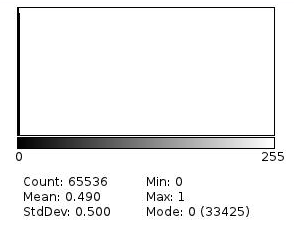
\includegraphics[scale=0.6]{qual/hist_ImageJVsCon.png} }
%%\caption{Grauwertdifferenz: ImageJ im Vergleich zur Ortsfaltung.
%%Rundungsabweichungen von max. einem Grauwert. Bild 30 fach verstärkt und
%%invertiert.}%
%%\label{figure_border_imageJ}
%%\end{figure}
  

\begin{figure}[htbp]
\framebox[\textwidth] 
{ 
\includegraphics[scale=1]{qual/diff_ConVsfCon_mal30.png}
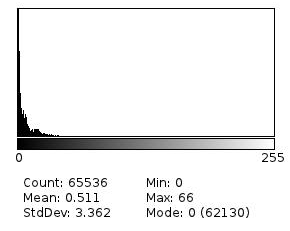
\includegraphics[scale=0.6]{qual/hist_ConVsfCon.png} }
\caption{Grauwertdifferenz: Die linke Abbildung zeigt kaum sichtbare
Randunterschiede der Faltung im Orts- und Frequenzbereich, sowie Rundungsdifferenzen
in der Bildmitte; Darstellung 30fach verstärkt und
invertiert, rechts: das Histogramm}%
\label{figure_border_convolve}
\end{figure}

%%\begin{figure}[htbp]
%%\makebox[\textwidth] 
%%{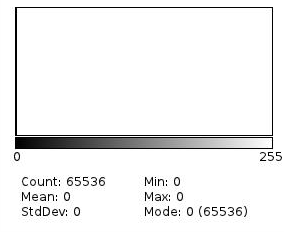
\includegraphics[scale=0.7]{qual/hist_BoxSepVsCon.png} }
%%\caption{Grauwertdifferenz: das Histogramm zeigt die Unterschiede zwischen
%%Ortsfaltung und separierten Boxfilter, inkl. Box 1D. keine Unterschiede}%
%%\label{figure_border_BoxSep}
%%\end{figure}

%%\begin{figure}[htbp]
%%\makebox[\textwidth] 
%%{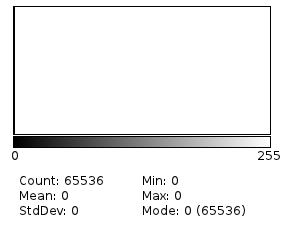
\includegraphics[scale=0.7]{qual/hist_Box2dVsCon.png} }
%%\caption{Grauwertdifferenz: das Histogramm zeigt die Unterschiede zwischen
%%zeilenweisen Boxfilters und der Ortsfaltung. keine Differenz}%
%%\label{figure_border_BoxnotSep}
%%\end{figure}


%%\begin{figure}[htbp]
%%\makebox[\textwidth] 
%%{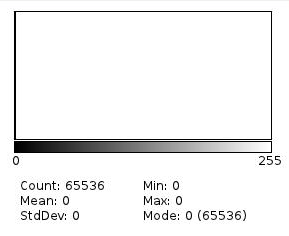
\includegraphics[scale=0.7]{qual/hist_listFilterConst_Vs_Con.png} }
%%\caption{Grauwertdifferenz zwischen Listenfilter, bzw. konstanten
%%Listenfilter und der Ortsfaltung. keine Unterschiede }%
%%\label{figure_hist_listFilter}
%%\end{figure}

%%\begin{figure}[htbp]
%%\makebox[\textwidth] 
%%{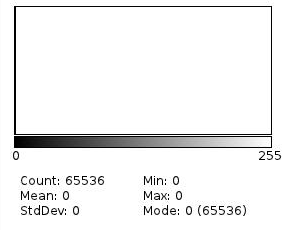
\includegraphics[scale=0.7]{qual/hist_genBoxVsCon.png} }
%%\caption{Grauwertdifferenz zwischen generischen Boxfilter und der Ortsfaltung.
%%Dazu wurden drei Teilkerne für den generischen Boxfilter erstellt. }%
%%\label{figure_hist_genBox}
%%\end{figure}


\begin{figure}[htbp]
\framebox[\textwidth] 
{
\includegraphics[scale=1]{qual/diff_CumVsBox.png} 
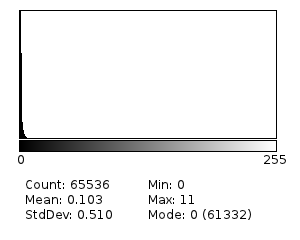
\includegraphics[scale=0.6]{qual/hist_CumVsBox.png} }
\caption{Grauwertdifferenz zwischen dem kumulierten Boxfilter und der Faltung im
Ortsbereich. Die Kerngröße nimmt zum Rand hin ab, so dass dort eine Differenz
entsteht; die Darstellung wurde invertiert und 30fach verstärkt}%
\label{figure_hist_kumuBox}
\end{figure}



\begin{figure}[htbp]
\framebox[\textwidth] 
{
\includegraphics[scale=1]{qual/simd_difference_fehler.png} 
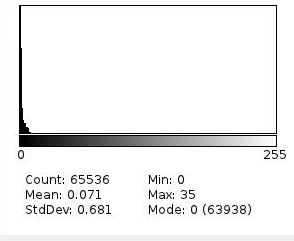
\includegraphics[scale=0.6]{qual/hist_simdVsCon.png} }
\caption{Grauwertdifferenz des Filters mit SIMD und ohne. 30fach verstärkt. Die
Randbedingung weicht leicht ab und Rundungsfehler in der Mitte sind zu erkennen. }%
\label{figure_hist_simd}
\end{figure}

\textbf{Lokalisierung}. Ein weiterer qualitativer Vergleich ist durch Prüfung
der Lokalisierungs\-genauigkeit möglich. In Abb. \ref{figure_lokalisierung}
wurde von ausgewählten Methoden jeweils der Punkt (103,103) farblich markiert. 
So ist eine einfache visuelle
Kontrolle der Lokalisierung möglich. Geschärft wurde jeweils mit RRRL bei einer
Unschärfe eins Boxfilter mit $7 \cdot 7$ px. Visuell lassen sich keine
Differenzen feststellen.

\begin{figure}[htbp]
\makebox[\textwidth] 
{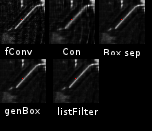
\includegraphics[scale=2]{qual/Lokalisierung.png}  }
\caption{Lokalisierungsgenauigkeit. Der Punkt (103,103) wurde jeweils rot
markiert. untersuchte Faltungen: F. im Frequenzbereich, Ortsbereich,
separierter Boxfilter, generischer Boxfilter und der Listenfilter.}%
\label{figure_lokalisierung}
\end{figure}

\subsubsection{Performancemessung}
Um die Laufzeit der einzelnen Faltungsroutinen zu vergleichen, wurden diese
einzeln gemessen und als Teil einer RL- sowie RRRL-Dekonvolution gemessen.

\textbf{Faltungsroutinen einzeln gemessen}. Es wurde jeweils das Bild mit dem
Kameramann (Abb. \ref{figure_camera}) mit einem Kern von $17 \cdot 17$ Pixeln
gefaltet. Das Diagramm aus Abb.\ref{figure_zeit_faltung} zeigt die gemessenen
Berechnungszeiten.
Folgende Parameter wurden gewählt:
\begin{itemize}
  \itemsep -1pt
  \item convolve: Ortsfaltung. Kern $17 \cdot 17$px
  \item listFilter: Listenfilter, kreisrunder Kern mit 213 Elementen
  Listengröße
  \item convolve SIMD: SSE-optimierte Ortsfaltung mit einem Kern von $20 \cdot
  20$ Pixel
  \item fconvolve: Faltung im Fourierbereich; die Kerngröße ist $17 \cdot 17$px
  \item genbox: generischer Boxfilter mit einem Lensblur von 17px Durchmesser.
  213 Pixel besetzt
  \item box2D nicht separiert: Kerngröße $17 \cdot 17$px
  \item box2D separiert: Kerngröße $17 \cdot 17$
  \item box2D kumuliert: Kerngröße von $17 \cdot 17$px.
  \item box1D: Motionblur in horizontaler Richtung mit 17px Unschärfe
\end{itemize}

Die Routinen "`listFilter"' sowie "`convolve SIMD"' sind stark von dem gewählten
Kern abhängig. Deshalb ist der direkte Vergleich zu den anderen Methoden
bei einer Kerngröße von $17 \cdot 17$px nicht möglich. Beim Listenfilter ist
weniger entscheidend, wie groß der Kern ist, sondern wieviel Pixel des Kerns
besetzt ($>0$) sind. Details werden später in der Performancemessung zum
Listenfilter genannt. Die optimierte Ortsfaltung mit SIMD ist ebenso vom Kern abhängig: Die
Kernlänge sollte stets ein Vielfaches von vier sein. Deshalb ist auch hier kein
Vergleich mit einer Kerngröße von $17 \cdot 17$px möglich. Beim SIMD-Verfahren
wurde deshalb eine Kerngröße von $20 \cdot 20$ gewählt. Näheres dazu dann im
Abschnitt zur Laufzeitmessung SIMD.

\begin{figure}[htbp]
\framebox[\textwidth] { 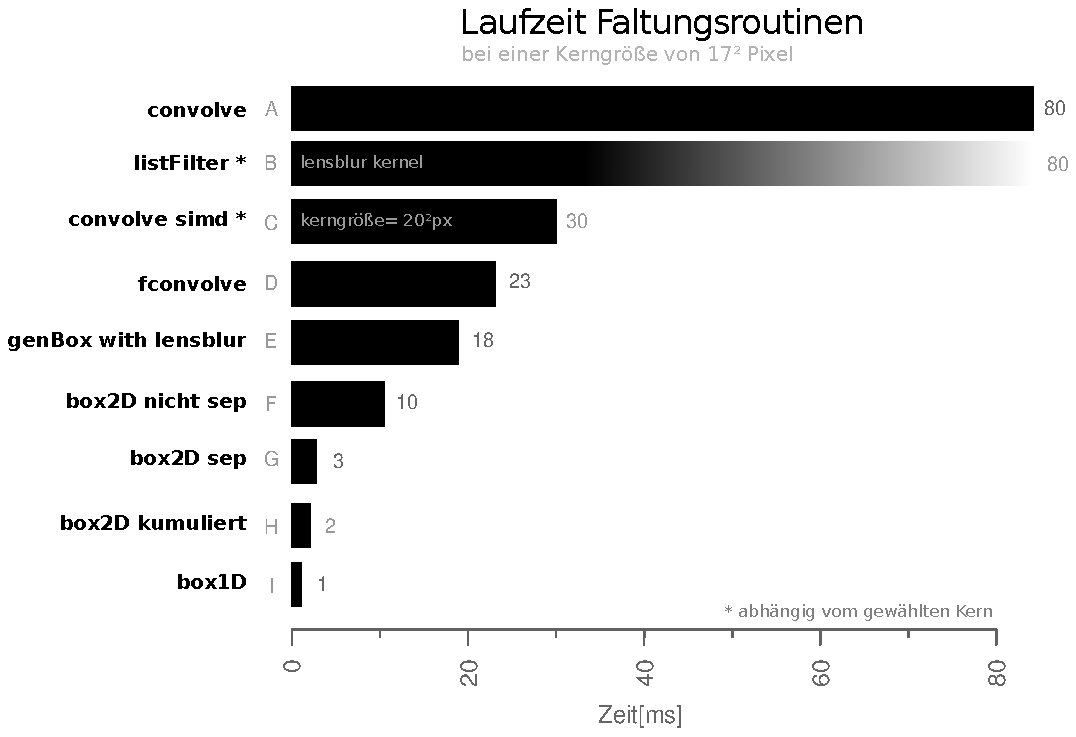
\includegraphics[scale=0.8]{faltungs_diagramm.pdf} }
\caption{Zeitbedarf der Faltungsroutinen}%
\label{figure_zeit_faltung}
\end{figure}  
  
 
\textbf{Laufzeit Listenfilter}
Wie bereits erwähnt, ist der Listenfilter nicht von der Kerngröße abhängig,
sondern von der Anzahl besetzter Pixel ($>0$). Wenn also ein Kern vorliegt, der
dünn besetzt ist, dh. wenn viele Pixel gleich Null sind, soll der Listenfilter
theoretisch schneller sein. Naheliegend scheint ein Vergleich Ortsfaltung zu
Listenfilter, wobei beim Ortsfilter die Kerngröße und beim Listenfilter die Listengröße
variiert. Das Diagramm von Abb. \ref{figure__list_vs_convolve} zeigt einen
solchen Vergleich.
Mit der Speicherorganisation in drei Komponenten (Kapitel \ref{chp:listFilter})
entsteht ein Overhead. Das bedeutet, dass die Ortsfilterung mit einem Kern von
200 Pixel schneller ist, als der Listenfilter mit 200 Elementen. Die Messung
zeigt: Die Ortfaltung braucht bei einem Kern von $1 \cdot 200$ Pixel etwa 48ms.
Der Listenfilter zeigt eine Laufzeit von 87ms (bei 200 Elementen). Daraus
resultiert ein Overhead von über 40 Prozent. Ein Vergleichsbeispiel: Wenn im
optimalen Fall ein diagonaler Bewegungsunschärfekern vorliegt, sind mit dem
Listenfilter nicht $10 \cdot 10$ Pixel zu berechnen (bei einer Kerngröße von $10
\cdot 10$px), sondern nur 10. Daraus resultiert in etwa ein Speedup um den
Faktor $6$ (inkl geschätzter Overhead).

Der konstante Listenfilter ist effizienter. Es müssen deutlich weniger
Gleitpunkt\-multiplikationen durchgeführt werden. Der konstante Listenfilter
benötigt für 200 Listenelemente 74ms. Das bedeutet einen Overhead von etwa 35
Prozent. Die Vorteil der Gleitpunkt-Additionen statt -Multiplikationen ist von
der verwendeten CPU abhängig.\\

  

\begin{figure}[htbp]
\makebox[\textwidth] { 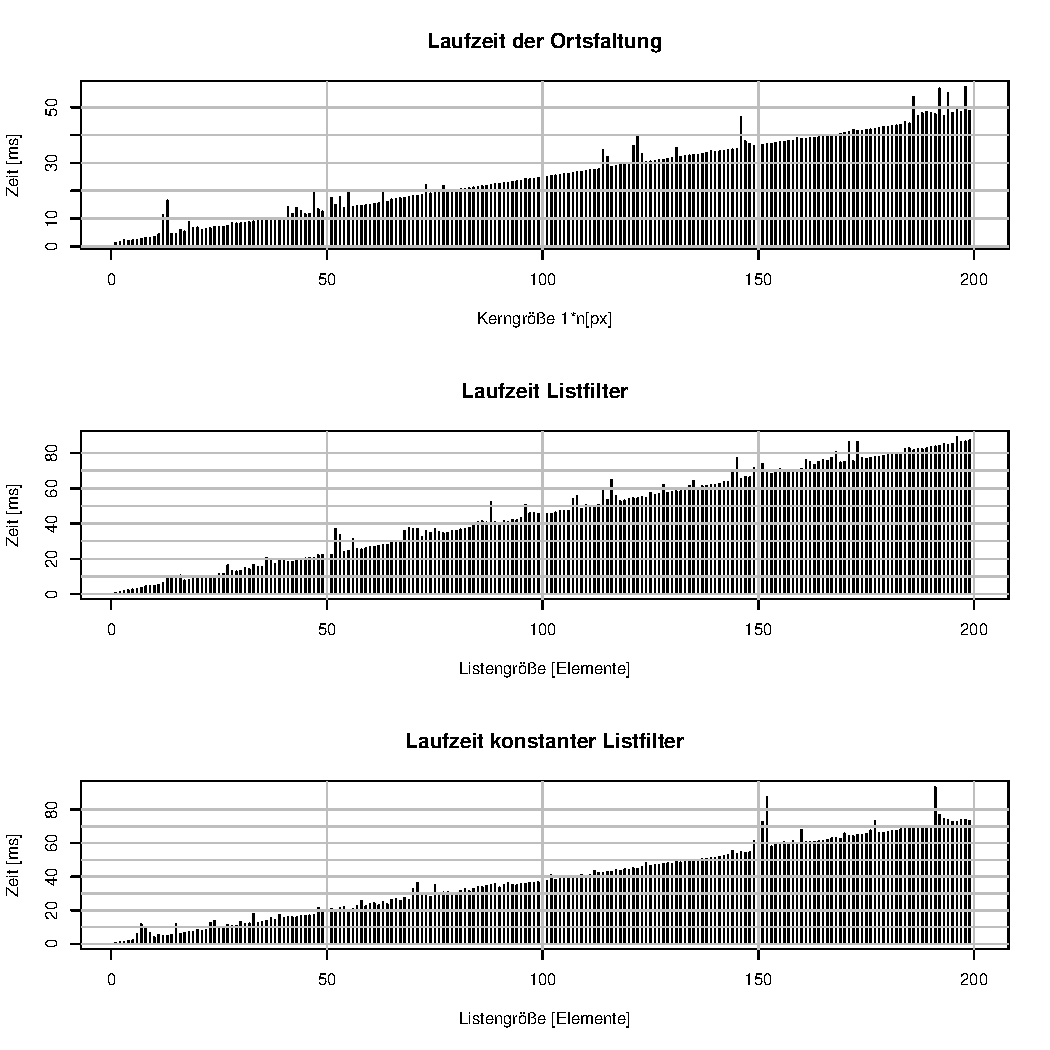
\includegraphics{listFilter_vs_convolve.pdf} }
\caption{Zeitbedarf der Faltungsroutinen Listfilter und Ortsfaltung}%
\label{figure__list_vs_convolve}
\end{figure}


\textbf{Laufzeit SIMD Ortsfaltung}. 
Wenn wir das Diagramm von Abb. \ref{figure_simd_vs_con} betrachten, können wir
die Laufzeit der SIMD-optimierten Ortsfaltung sehen. Die auftretenden Peaks
zeigen das nicht-deterministische Verhalten des Betriebssystems: Ubuntu ist kein
Echtzeitbetriebssystem und garantiert deshalb auch nicht die gleichmäßige
Priorisierung eines Threads. 

Außerdem: Die grüne Linie, also die optimierte Version zeigt stufenhafte
Sprünge in Vierer-Schritten. Hier ist anzunehmen, dass die CPU bei
vier-alignierter Kernlänge alle Rechenoperationen auf den SSE-Registern
druchführen kann. Bei Kerngrößen, welche nicht durch vier teilbar sind, müssen
immer ein, zwei oder drei Rechenschritte auf den normalen CPU-Registern
einzeln ausgeführt werden. Die nächste Frage stellt sich also: Wie ist das
Verhalten, wenn der Kern nicht die Form $1 \cdot n$ hat, sondern realistischer\-weise 
die Dimension $n \cdot n$? Ist eine Verschlechterung der Performance zu
erwarten? Theoretisch sind bei einem Kern von beispielsweise $7 \cdot 7$ Pixel
mindestens $3 \cdot 7 = 21$ nicht parallisierte Rechenschritte nötig. Den
Unterschied zeigt Abb. \ref{figure_simd_vs_con_quadtrat}. Die ungünstige
Speicherausrichtung scheint demnach keinen großen Einfluss auf die Performance
zu haben. Das unregelmäßige Ansteigen kann aber mit der Speicherauslagerung in
Zusammenhang gebracht werden.



\begin{figure}[htbp]
\makebox[\textwidth] { 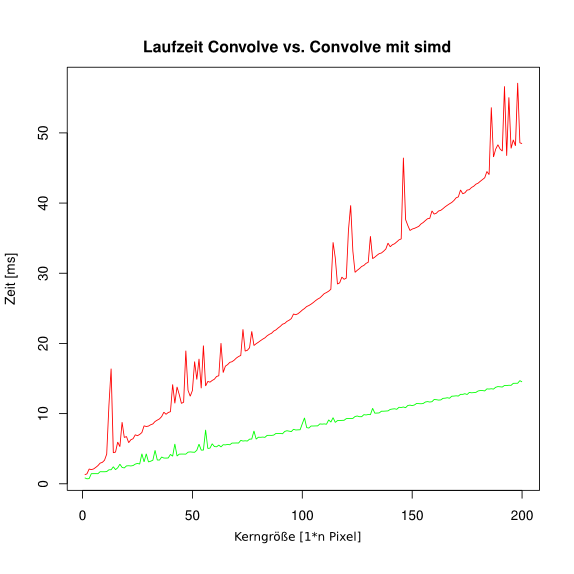
\includegraphics[scale=0.7]{simd_vergleich_lin.png} }
\caption{Zeitbedarf der gewöhnlichen Ortsfaltung und der SIMD-optimierten.
Kerngröße steigt in der Form $1 \cdot n$ linear an}%
\label{figure_simd_vs_con}
\end{figure}

\begin{figure}[htbp]
\makebox[\textwidth] { 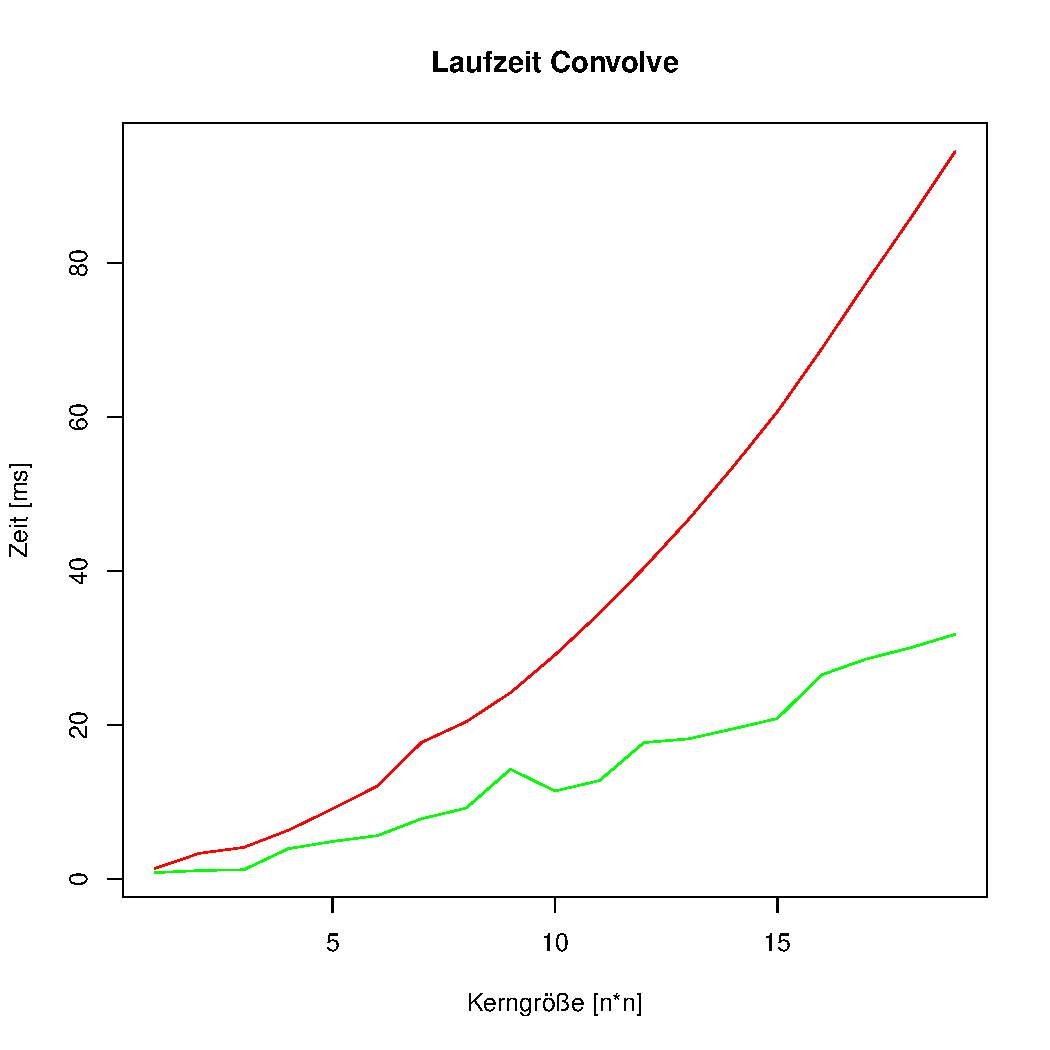
\includegraphics[scale=0.7]{simd_vergleich_quadrat.pdf} }
\caption{Zeitbedarf der gewöhnlichen Ortsfaltung und der SIMD-optimierten.
Kerngröße steigt in der Form $n \cdot n$ quadratisch an}%
\label{figure_simd_vs_con_quadtrat}
\end{figure}

\textbf{Faltungsroutinen mit Richardson-Lucy-Dekonvolution (RL)}.
Die vorgestellten Faltungsroutinen wurden in den RL-Algorithmus integriert und
getestet. Die nachfolgenden Abbildungen zeigen den Zeitbedarf der gesamten
Dekonvolution bei 100 Iterationen. Die Abb. \ref{figure_zeit_rl} zeigt die
Ergebnisse nach Kerngrößen geordnet. Die Abb. \ref{figure_zeit_rl_umgruppiert}
zeigt dieselben Ergebnisse, aber nach Faltungsmethoden gruppiert. Nachfolgend
werden die Parameter der jeweiligen Faltungsfunktionen aufgelistet:
\begin{itemize}
  \itemsep -1pt
  \item convolve: Ortsfaltung
  \item listFilter const: Listenfilter mit Lensblur-Kern; 
  Listengröße $\approx d^{2}/4 \cdot \pi$ Elemente. $d = 17px, 11px, 9px$
  \item convolve SIMD: Ortsfaltung mit SSE-Optimierung
  \item fconvolve: Faltung im Fourierbereich
  \item genBox: Faltung mit generischem Boxfilter. lensblur, dh. kreisrunder
  Kern. $d^{2}/4 \cdot \pi$ Elemente
  \item box2D nicht separiert: Boxkern mit jeweiliger Kerngröße.
  \item box2D kumuliert: kumulierter Boxfilter
  \item box2D separiert: Boxkern mit jeweiliger Kerngröße.
  \item box1D: Boxkern mit $1 \cdot n$ Pixel. $d = 17,11,9$
\end{itemize}

Die Ergebnisse der Ortsfaltung, Faltung im Frequenzbereich und des Boxfilters
sind bekannt und dienen an dieser Stelle als Vergleich. Der 1D-Boxfilter ist
bekannterweise der schnellste Filter. Er arbeitet aber auch mit dem speziellsten
Filterkern: der konstanten Bewegungsunschärfe in horizontaler, bzw. vertikaler
Richtung. Wie alle Boxfilter ändert er sich mit der Kerngröße nicht.
Die Faltung im Fourierbereich ist ebenso von der Größe des Kerns unabhängig.


\begin{figure}[htbp]
\makebox[\textwidth] { 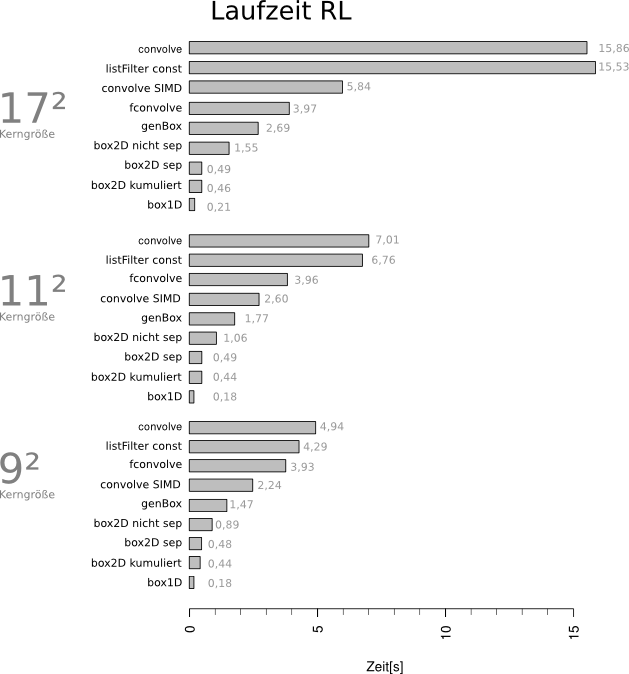
\includegraphics[scale=0.9]{rl_messung.png} }
\caption{Zeitbedarf RL mit verschiedenen Faltungsroutinen, gruppert nach
Kerngröße, 100 Iterationen}%
\label{figure_zeit_rl}
\end{figure}
 
\begin{figure}[htbp]
\makebox[\textwidth] { 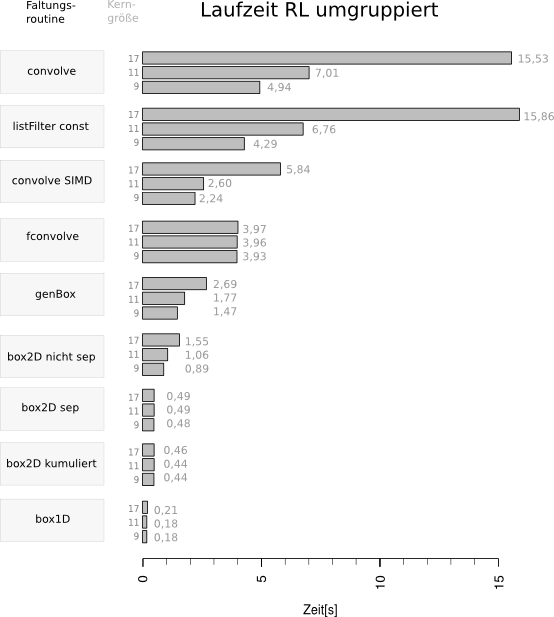
\includegraphics[scale=0.9]{rl_messung_umgruppiert.png} }
\caption{Zeitbedarf RL mit verschiedenen Faltungsroutinen, gruppert nach
Faltungsroutinen, 100 Iterationen}%
\label{figure_zeit_rl_umgruppiert}
\end{figure}
 
\textbf{Faltungsroutinen mit RRRL}.
Bei der Faltung mit dem RRRL zeigen sich ähnliche Ergebnisse, wie bei der
Faltung mit dem RL-Algorithmus. Hier sollte erwähnt werden, dass eine dritte
Faltung durchgeführt werden muss. Das qualitative Ergebnis des RRRL ist 
mit dem des RL-Algorithmus nicht uneingeschränkt vergleichbar, da der RRRL
eine zusätzliche Regularisierung zur Verfügung stellt. 
Als Parameter wurden gewählt: $\alpha = 0.000001$ und $\epsilon =
0.1$. Der RRRL wurde ebenfalls bei 100
Iterationen getestet.
Hier fällt sofort auf, dass das Minimum des 1D-Boxfilters nicht so deutlich hervortritt, als beim
RL. Der Grund dafür liegt im Mehraufwand der Berechung: Beim RRRL müssen noch
zusätzliche Werte (zb. $\Phi$) berechnet werden und der Anteil der Faltung an
der gesamten Rechenzeit ist nicht mehr so hoch.


\begin{figure}[htbp]
\makebox[\textwidth] { 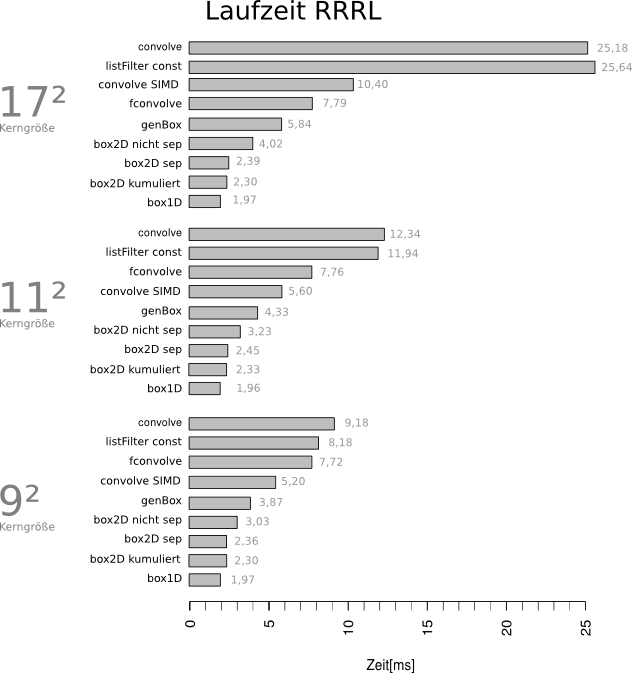
\includegraphics[scale=0.9]{rrrl_messung.png} }
\caption{Zeitbedarf RRRL mit verschiedenen Faltungsroutinen, Parameter: 100
Iterationen, Alpha = 0.000001 , Epsilon = 0.1 }%
\label{figure_zeit_rrrl}
\end{figure}







 
\subsection{Messergebnisse der Konvergenzanalyse}

\textbf{Messungen bei 100 Iterationen und verschiedener Optimierungsparametern.}
Berechnet wurde das Bild des Kameramanns (Abb. \ref{figure_camera}) mit einem Lensblur von 17px Durchmesser. In zwei Messreihen wurden der optimierte
RL und der optimierte RRRL mit der gewöhnlichen Ortsfaltung verwendet. 
Alle 10 Iterationen wurde die Faltung ohne Optimierung berechnet.
Im Interfall $0.01\ldots0.09$ treten jeweils geringe qualitative Einbußen statt.
Im Intervall $0.1\ldots0.5$ ist das Ergebnis visuell bereits deutlich
verschlechtert. Hier sind immerhin deutliche Einsparungen in der Rechenzeit
möglich und zwar bis zu einem Fünftel der ursprünglichen Rechenzeit
(Tab. \ref{tab:konv_time_SNR_RL}).
\\
Die Tabelle \ref{tab:konv_time_SNR_RRRL} zeigt die Messreihe mit dem
RRRL-Algorithmus. Als Regularisierungs\-parameter wurden gewählt: 
$\alpha = 0.000001, \epsilon = 0.1$.

\textbf{Rechenaufwand der zusätzlichen Kontrollstrukturen - der Overhead.}
Die optimierte Version der Faltungsroutine beinhaltet eine if-Klausel. Diese
Abfrage prüft, ob der Schwellwert des jeweiligen Pixels erreicht wurde. 
Diese Kontrollstrukturen bringen also einen Overhead mit sich. Zur
Veranschaulichung beinhaltet hier jede Tabelle zwei Vergleichswerte der
nicht optimierten Version:
\begin{itemize}
  \itemsep -1pt
  \item performRL/performRRRL: Hier wurde die ursprüngliche Version, ohne
  Optimierung und ohne Kontrollstrukturen gemessen (ohne Overhead)
  \item $k=-10$: Hier wurde die optimierte Version mit Kontrollstrukturen
  gemessen. Das $k$ wurde so niedrig gewählt, dass alle Pixel in jeder Iteration
  voll gefaltet wurden (also mit Overhead).
\end{itemize}
Das Ergebnis zeigt, dass praktisch kein Overhead entsteht! Auffällig ist, dass
die Zeiten der ursprünglichen Routine und des optimierten Algorithmus gleich
sind. Das ist optimal, weil bereits bei einem kleinen k-Wert die Rechenzeit
verkürzt wird.

\textbf{Anzahl der ignorierten Pixel.} Um ein Maß für die Optimierung zu finden
wurde ausgewertet, wieviele Pixel bei der Faltung übersprungen, also nicht
gefaltet worden sind. Die Werte stehen jeweils in der zweiten Spalte in den
Tabellen \ref{tab:konv_time_SNR_RL}, \ref{tab:konv_time_SNR_RRRL} und
\ref{tab:konv_time_SNR_RL_500}. Die Diagramme in Abb. \ref{figure_konv_ratio}
zeigen den Verlauf dieses Anteils. Der Verlauf des oberen Diagramms nähert sich
auf den Endwert von $0.23$ ein (siehe Tab. \ref{tab:konv_time_SNR_RL_500}). Das
heißt, dass das Verhältnis der gefalteten Pixel zu den ignorierten Pixeln bei
$0.23$ liegt. In anderen Worten kann man also sagen, dass hier nur ein
Viertel aller Pixel tatsächlich berechnet wurden und die anderen ignoriert. Daraus
entsteht laut Tabelle \ref{tab:konv_time_SNR_RL_500} aber dann eine
Beschleunigung um das Fünffache.

\begin{table}[h]
\begin{center}
\begin{tabular}{ | l | l | l | l | l |}
\hline
k-Wert 				 &	Verhältnis Faltung 	& Zeit [s] & SNR[dB] & Speedup \\ \hline
performRL		 	 & 		$1/0$			& 	15.43 & 17.25& 	1.0 	\\ \hline
-10 			 	 & 		$1/0$			& 	15.51 & 17.25& 	1.0 	\\ \hline
0.01				 & 		3.74			&	12.29 & 17.25    &  1.27\\
0.02				 & 		2.04			&	10.48 & 17.25    & 	1.49\\
0.03				 & 		1.46			&	9.34  & 17.24    & 	1.66\\
0.04				 &		1.16			&	8.42  & 17.23    & 	1.84\\
0.05				 & 		0.97			&	7.76  & 17.21    & 	2.00\\
0.06				 & 		0.85			&	7.23  & 17.18    & 	2.15\\ 
0.07				 & 		0.75			&	6.79  & 17.16    & 	2.28\\
0.08				 & 		0.68			&	6.47  & 17.13    & 	2.40\\
0.09				 & 		0.63			&	6.11  & 17.11    & 	2.54\\
0.1					 & 		0.59			&	5.86  & 17.08    & 	2.65\\
0.2					 &		0.37			&	4.31  & 16.87    & 	3.60\\
0.3					 &		0.28			&	3.59  & 16.69    & 	4.32\\
0.4					 & 		0.24			& 	  3.16  & 16.52    & 	4.91\\
0.5					 & 		0.22			&	2.89  & 16.37    & 	5.37\\ \hline
                     
blurred image	&		  & 12.86 & \\
\hline
\end{tabular}
\caption{RL mit Optimierung: Die Laufzeiten für verschiedene k-Werte und
Signal-Rausch-Verhältnisse, 100 Iterationen}
\label{tab:konv_time_SNR_RL}
\end{center}
\end{table}



\begin{table}[h]
\begin{center}
\begin{tabular}{ | l | l | l | l | l |}
\hline
k-Wert 			&	Verhältnis Faltung 	& Zeit [s] & SNR[dB] & Speedup \\ \hline
perform RRRL	& 		$1/0$			& 	24.79 & 16.67    & 	1	\\ \hline
-10				& 		$1/0$			& 	24.83 & 16.67    & 	1	\\ \hline
0.01			& 		4.36			&	20.55 & 16.67    &  1.20\\
0.02			& 		2.41			&	18.08 & 16.66    & 	1.37\\
0.03			& 		1.72			&	16.50 & 16.66    & 	1.50\\
0.04			&		1.39			&	15.12 & 16.65    & 	1.63\\
0.05			& 		1.18			&	14.34 & 16.64    & 	1.72\\
0.06			& 		1.04			&	13.46 & 16.61    & 	1.84\\ 
0.07			& 		0.94			&	12.90 & 16.59    & 	1.92\\
0.08			& 		0.86			&	12.36 & 16.56    & 	2.00\\
0.09			& 		0.80			&	11.90 & 16.53    & 	2.08\\
0.1				& 		0.76			&	11.66 & 16.52    & 	2.12\\
0.2				&		0.53			&	9.64  & 16.37    & 	2.57\\
0.3				&		0.46			&	8.81  & 16.29    & 	2.81\\
0.4				& 		0.42			&   8.38  & 16.21    & 	2.95\\
0.5				& 		0.39			&	8.03  & 16.10    & 	3.08\\ \hline
blurred image	&		 				& 		  & 12.86 	 & \\
\hline
\end{tabular}
\caption{RRRL mit Optimierung: Die Laufzeiten für verschiedene k-Werte
und Signal-Rausch-Verhältnisse, 100 Iterationen, $\alpha = 0.000001, \epsilon = 0.1$}
\label{tab:konv_time_SNR_RRRL}
\end{center}
\end{table}


\textbf{Nähere Betrachtung bei 500 Iterationen.}
Der RL wurde nun bei 500 Iterationen getestet. Bei dieser Iterationszahl ist das
Ergebnis der Schärfung bereits sehr deutlich zu sehen. Die Tabelle zeigt eine
Übersicht der Messung.

\begin{table}[h]
\begin{center}
\begin{tabular}{ | l | l | l | l | l |}
\hline
k-Wert 				& Verhältnis Faltung	& Zeit [s] 	& SNR[dB] & Speedup \\ \hline
perfornRL		 	&		$1/0$				& 	77.5 	& 19.33   & 	1	\\ \hline
-10				 	&		$1/0$				& 	77.9 	& 19.33   & 	1	\\ \hline
0.01				&		1.15				&	42.2 	& 19.29   &  	1.85\\
0.1					&		0.23				&	15.2 	& 18.40   & 	5,13\\ \hline

blurred image		&		  					& 			&	12.86 & 		\\
\hline
\end{tabular}
\caption{RL bei 500 Iterationen.}
\label{tab:konv_time_SNR_RL_500}
\end{center}
\end{table}
 
\begin{figure}[htbp]
\makebox[\textwidth] {
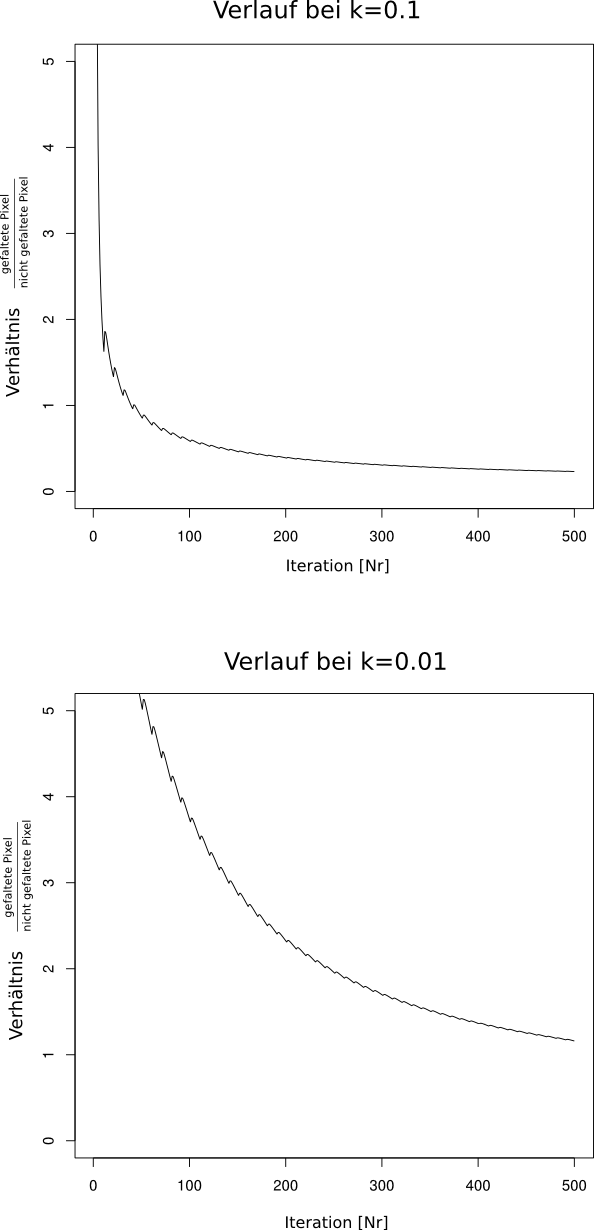
\includegraphics[scale=0.6]{ratio.png} }
\caption{RL: Anteil gefalteter Pixel, 500 Iterationen, bei k=0.01 und k=0.1}%.
\label{figure_konv_ratio}
\end{figure}

\begin{figure}[h]
\makebox[\textwidth] {
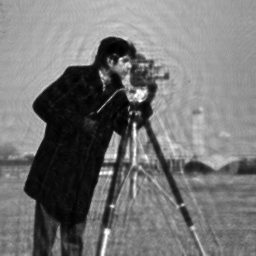
\includegraphics[scale=1.0]{konv/out_ohne.png} }
\caption{RL ohne Optimierung, 500 Iterationen}%.
\label{figure_konv_ohne}
\end{figure}

\begin{figure}[h]
\makebox[\textwidth] {
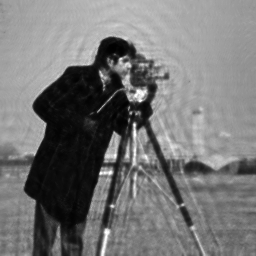
\includegraphics[scale=1.0]{konv/out_0_01_500.png} }
\caption{RL mit Optimierung, 500 Iterationen, $k = 0.01$}%.
\label{figure_konv_k0_01}
\end{figure}


\begin{figure}[h]
\makebox[\textwidth] {
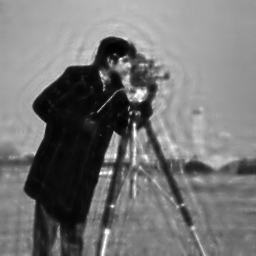
\includegraphics[scale=1.0]{konv/out_0_1_500.png} }
\caption{RL mit Optimierung, 500 Iterationen, $k = 0.1$}%
\label{figure_konv_k0_1}
\end{figure}






\newpage

%%%%%%%%%%%%%%%%%%%%%%%%%%%%%%%%%%%%%%%%%%%%%%%%%%%%%%%%%%%%%%%%%%%%%
\section{Diskussion}

In der Arbeit wurden neue Methoden zur Faltung mit speziellen Faltungskernen
entwickelt. Diese Faltungsroutinen dienen als Werkzeug für die Berechnung
iterativer Dekonvolutions\-verfahren, und zwar des Richardson-Lucy
\cite{richardson}, \cite{lucy} und des robust regularisierten
Richardson-Lucy-Algorithmus \cite{rrrl}. Ebenso konnte eine Möglichkeit gefunden werden, bei der sich die Berechnung auf die relevanten Pixel begrenzen läßt. So
kann Rechenzeit gespart und der Dekonvolutionsalgorithmus beschleunigt werden.
Im Folgenden werden die Vor- und Nachteile der entwickelten Verfahren
aufgezeigt.

\subsection{Eigenschaften der entwickelten Faltungsroutinen}
Bei den neu entwickelten Filtern wurden spezielle Faltungskerne zugrunde gelegt.
Die Methoden wurden auf einer Plattform getestet, sie wurden aber
nicht hardware\-spezifisch optimiert. Das bedeutet, dass der Einsatz weniger von
der verwendeten Hardware abhängig ist, sondern vielmehr vom vorliegenden
Faltungskern. Mit dem SIMD-optimierten Ortsfilter wurde außerdem eine Methode
implementiert, die eine parallelisierte Berechnung ermöglicht. Der Vorteil
der Parallelisierung ist, dass der Filter vom Faltungskern unabhängig ist.
Jedoch ist für die Implementierung der parallelisierten Berechnung eine bestimmte 
Hardwareplattform (mit mehreren Rechenkernen bzw. speziellen Befehlssätzen wie
SSE) notwendig. Wenn die Implementierung dann aber an die jeweilige
Hardwareplattform angepasst wird, sind sehr effiziente Implementierungen
möglich, wie der Vergleich der Ortsfaltung mit der SIMD-optimierten Ortsfaltung
gezeigt hat. Die meisten hier entwickelten Verfahren sind jedoch nicht weiter
parallelisierbar. Deshalb sollte zuerst die Verwendung der gewöhnlichen
Ortsfaltung und der Faltung im Fourierbereich mit angemessener Anpassung an die
Hardware in Betracht gezogen werden. Falls eine aufwendige Anpassung an die
Hardware nicht möglich oder gewünscht ist, kommt dann aber eine der
folgenden Methoden in Frage:

Mit dem generischen Boxfilter wurde eine Methode gefunden, mit der sich
verschiedene Faltungskerne effizient berechnen lassen. Die Rechengeschwindigkeit
ist bei einer Kerngröße von $17 \cdot 17$px höher als die implementierte
Faltung im Fourierbereich. Die Voraussetzung für die
Verwendung des generischen Boxfilters ist, dass die Pixel des zugehörigen
Faltungskerns in einer Zeile zusammenhängen und konstant sind. Dann lassen sich
verschiedene Kerne falten: Eine typische Anwendung wird der Lensblurfilter sein. Der Kern
des Lensblurfilter ist ein gefüllter Kreis und modelliert die Unschärfe durch
Defokussierung. In der Fotografie kommt das Problem der fehlerhaften
Fokussierung sehr häufig vor und könnte deshalb eine typische Anwendung sein.
Häufig ist die Form der Blende nicht exakt kreisförmig. Auch diesen Fall kann
der Filter abdecken und Faltungen mit konvexen Polygonen berechnen.

Der entwickelte Listenfilter kann mit allen Faltungskernen umgehen. Allerdings
bringt er einen Mehraufwand in der Berechnung mit sich. Die Verwendung des
Filters lohnt sich erst, wenn weniger als halb so viele Pixel des Kerns besetzt
sind (Der gemessene Overhead ist etwa 50\% gegenüber der Ortsfaltung). Ein
typischer Anwendungsfall für diesen Listenfilter kann die unregelmäßige
Bewegungsunschärfe sein. Hier kann der Filter seine Stärke ausspielen, weil die
PSF der Bewegungsunschärfe idR. dünn besetzt ist.

Mit dem kumulierten 2D-Boxfilter wurde eine Methode entwickelt, mit der sich der
Boxfilter noch schneller berechnen läßt. Der kumulierte Boxfilter ist knapp
schneller als der separierte. Dieser Zeitvorteil kann bei steigender Bildgröße
noch deutlicher hervortreten. 



\subsection{Vor- und Nachteile der konvergenzorientierten Optimierung}
Die iterativen Dekonvolutionsverfahren RL und RRRL konnten durch Selektion
einzelner relevanter Pixel beschleunigt werden. Dabei konnte bei 500 Iterationen
die Rechen\-geschwindigkeit um das Fünffache erhöht werden. Natürlich bringt das
eine Verschlechterung des Ergebnis mit sich. Dennoch kann bei der Wahl des
geeigneten Parameter ein Kompromiss zwischen Qualität und Performance
individuell gewählt werden. Für manche Anwendung kann es sinnvoll sein, eine
rasche und grobe Vorberechung auszuführen. Gleichzeitig ist die Beschleunigung
ohne großer Qualitätseinbußen um den Faktor 2 möglich. Die Anwendungen können also
vielfältig sein. Seine besondere Stärke spielt die konvergenzoptimierte Version
 in Verbindung mit dem Listenfilter aus. Speziell der
Listenfilter ermöglicht die isolierte Faltung einzelner ausgewählter Pixel. Der
konvergenzoptimierte RL/RRRL mit dem Listenfilter ausgeführt kann demnach
Beschleunigungen über das Fünffache gegenüber der gewöhnlichen
Ortsfaltung bringen.
 
%%\subsection{Ausblick}
%%Die vorgestellten Faltungsroutinen ermöglichen die Beschleunigung von RL- und
%%RRRL-Algorithmen. Gleichzeitig wurden diese iterativen Algorithmen angepasst
% und damit wird es möglich einen Kompromiss zwischen Qualität und Performance
%%zu finden. Der begrenzende Faktor ist bei Dekonvolutionsverfahren oft die
% Zeit.
%%Wenn die Performance dieser Verfahren verbessert wird, könnten die
%%Dekonvolutionsverfahren in neue Anwendungen gebracht werden. Beispielsweise in
%%der industriellen Bildverarbeitung oder bei tragbaren Kameras.

\newpage
 
\section{Zusammenfassung/Abstract}
\textbf{Deutsch}

Itertive Dekonvolutionsverfahren ermöglichen die Rekonstruktion von
unscharfen Bildern. Häufige Ursachen von Unschärfe sind ungünstige
Lichtverhältnisse, zu schnelle Bewegung oder fehlerhafte Fokussierung. 
Wenn die genaue Form und das Ausmaß der Unschärfe
bekannt sind, kann das Bild mit Dekonvolutionsalgorithmen geschärft werden.
Die iterativen Verfahren wie der Richardson-Lucy-Algorithmus oder der robust
regularisierte Richardson-Lucy-Algorithmus sind jedoch rechenintensiv und
benötigen oft mehrere hundert Iterationen, um ein hochwertiges Ergebnis zu
berechnen. Die meiste aufgewendete Rechenzeit wird dabei in die Faltung der
Zwischenergebnisse investiert. Dazu wurden nun mehrere Verfahren vorgestellt,
die eine effiziente Berechnung bei speziellen Faltungskernen ermöglichen. Diese
speziellen Faltungskerne stehen in direktem Bezug zu der entstandenen Unschärfe:
Der vorgestellte Lensblur-Filter ermöglicht so die effiziente Dekonvolution von
defokussierten Bildern. Die Form der Filtermaske kann dabei an die exakte Form
der Blendenöffnung angepasst werden. Der Listenfilter bietet eine schnelle
Berechnung von unregelmäßigen Bewegungsunschärfen. Speziell, wenn die Unschärfe
diagonal verläuft, erzielt der Filter die beste Performance. Der Rechenzeit ist
dabei linear abhängig von der Anzahl der besetzten Pixel, mit einem gemessenen
Overhead von 50\%. Das bedeutet bei einem diagonal verlaufenden Unschärfekern
von $10 \cdot 10$px eine Beschleunigung um mehr als den Faktor 6 im Vergleich
zu der Faltung im Ortsbereich.
Neben der Optimierung der Faltungsopertionen wurde ein weiterer Ansatz verfolgt:
Bei der Iteration des Richardson-Lucy (RL) und robust regularisierten RL ändern
sich manche Pixel stärker. Andere Pixel werden durch die Dekonvolution kaum
verändert. Das sind etwa Pixel, die in einer homogenen Umgebung liegen. Im
vorgestellten Verfahren wurden anhand zweier verschiedener Maßzahlen 
(Varianz und Grauwertdifferenz) die relevanten Pixel selektiert. Die
Berechnung wurde nur auf die selektierten Pixel angewandt. So konnte die
Rechenzeit um mehr als den Faktor 5 verringert werden. Dabei ist es möglich,
einen Kompromiss zwischen Qualität und Effizienz durch entsprechende Wahl des
Schwellwerts zu finden.
\\

\textbf{English}
Iterative deconvolution methods allow to reconstruct unsharp images.
Frequent causes of unsharp images are bad lighting conditions, fast movement or wrong focussing. These unsharp images can be sharpened with deconvolution 
algorithms, if the blurring parameters are known. The deconvolution algorithms 
Richardson-Lucy and the robust regularized Richardson Lucy are such methods. 
But for a high quality result, they require over hundred iterations, 
so that the calculation time becomes the limiting factor. The main time is spent 
on convolution. This thesis show some new methods for convolving images with special 
convolution kernels. The kernels are directly associated to the type of blurring, for 
example the lens blur kernel. It describes the blur, that comes along with images which
 have a wrong focus. The developed filter performs a convolution with this lens blur 
 kernel even faster than the convolution in frequency domain with a FFT. 
The fast lens blur filter can be adopted to the exact shape of the aperture.
Another special filter that was introduced is the so called list filter. 
  It allows the fast convolution with kernels, in which most grey values are zero. 
  Especially with motion blurs that drifts diagonally, this filter is most effective. 
  The calculation time of the list filter depends on the number of kernel pixels 
  that are not null. So in case of a diagonal motion blur, the list filter only 
  calculates $10$ Pixel instead of $10 \cdot 10$ Pixel. This causes an acceleration 
  of six times with an already included calculation overhead of 50\%.

With the mentioned convolution methods an optimized version of the Richardson-Lucy 
(RL) and the robust regularized RL algorithms have been introduced, with the following 
approach: Some pixels may not be changed during the convolution. The neighbor pixels of 
that ones are mostly uniform. The introduced technique performs the convolution only on 
the affected pixels. That selected pixels have been identified with two values: 
The variance and the difference of the grey values. So the calculation time could be 
accelerated with a factor of 5 compared to a standard space domain convolution. This 
optimization of course affects the quality. But the user can find a trade-off in quality 
and performance, simply with adjusting the threshold.






\newpage
\listoffigures 
\addcontentsline{toc}{section}{Abbildungsverzeichnis} 

\newpage
\listoftables
\addcontentsline{toc}{section}{Tabellenverzeichnis} 

\lstlistoflistings

\newpage
\bibliography{references}
\addcontentsline{toc}{section}{Literaturverzeichnis}
\bibliographystyle{plain}


\newpage 
Lebenslauf / CV

\addcontentsline{toc}{section}{Eidesstattliche Erklärung}




(kurzer tabellarischer Lebenslauf, max. eine Seite)
(Am Ende der gesamten Arbeit:)
Hiermit erkläre ich an Eides statt, die Arbeit selbständig verfasst und keine anderen
als die angegebenen Hilfsmittel verwendet zu haben.


%%\subsection{Another subtitle}
\end{document}
